%%%%%%%%%%%%%%%%%%%%%%%%%%%%%%%%%%%%%%%%%
% Classicthesis Typographic Thesis
% LaTeX Template
% Version 1.0 (23/4/12)
%
% This template has been downloaded from:
% http://www.LaTeXTemplates.com
%
% Original author:
% AndrŽ Miede (http://www.miede.de)
%
% License:
% CC BY-NC-SA 3.0 (http://creativecommons.org/licenses/by-nc-sa/3.0/)
%
% General Tips:
% 1) Make sure to edit the classicthesis-config.file
% 2) New enumeration (A., B., C., etc in small caps): \begin{aenumerate} \end{aenumerate}
% 3) For margin notes: \marginpar or \graffito{}
% 4) Do not use bold fonts in this style, it is designed around them
% 5) Use tables as in the examples
% 6) See classicthesis-preamble.sty for useful commands
%
%%%%%%%%%%%%%%%%%%%%%%%%%%%%%%%%%%%%%%%%%

%----------------------------------------------------------------------
%	PACKAGES AND OTHER DOCUMENT CONFIGURATIONS
%----------------------------------------------------------------------

\documentclass[
		openright,titlepage,numbers=noenddot,headinclude,%1headlines,
                footinclude=true,cleardoublepage=empty,
                BCOR=5mm,paper=a4,fontsize=12pt, % Binding correction, paper type and font size
                ngerman,american, % Languages
                ]{scrreprt} 
                
% Includes the file which contains all the document configurations and packages - make sure to edit this file
%%%%%%%%%%%%%%%%%%%%%%%%%%%%%%%%%%%%%%%%%
% Thesis Configuration File
%
% The main lines to change in this file are in the DOCUMENT VARIABLES
% section, the rest of the file is for advanced configuration.
%
%%%%%%%%%%%%%%%%%%%%%%%%%%%%%%%%%%%%%%%%%

%----------------------------------------------------------------------------------------
%	DOCUMENT VARIABLES
%	Fill in the lines below to enter your information into the thesis template
%	Each of the commands can be cited anywhere in the thesis
%----------------------------------------------------------------------------------------

% Remove drafting to get rid of the '[ Date - classicthesis version 4.0 ]' text at the bottom of every page
\PassOptionsToPackage{eulerchapternumbers,listings, pdfspacing, subfig,beramono,eulermath,parts}{classicthesis}
% Available options: drafting parts nochapters linedheaders eulerchapternumbers beramono eulermath pdfspacing minionprospacing tocaligned dottedtoc manychapters listings floatperchapter subfig
% Adding 'dottedtoc' will make page numbers in the table of contents flushed right with dots leading to them

\newcommand{\myTitle}{Agents: Investigating environment perception\xspace}
\newcommand{\mySubtitle}{MSc Project Report\xspace}
\newcommand{\myDegree}{Doktor-Ingenieur (Dr.-Ing.)\xspace}
\newcommand{\myName}{Luiz Filipe Polimeno Abrahao\xspace}
\newcommand{\myProf}{Put name here\xspace}
\newcommand{\myOtherProf}{Put name here\xspace}
\newcommand{\mySupervisor}{Dr Thrishantha Nanayakkara\xspace}
\newcommand{\myFaculty}{King's College London\xspace}
\newcommand{\myDepartment}{Engineering Department\xspace}
\newcommand{\myUni}{University of London\xspace}
\newcommand{\myLocation}{London, United Kingdon\xspace}
\newcommand{\myTime}{September 2012\xspace}
\newcommand{\myVersion}{Draft 2\xspace}

%----------------------------------------------------------------------------------------
%	USEFUL COMMANDS
%----------------------------------------------------------------------------------------

\newcommand{\ie}{i.\,e.}
\newcommand{\Ie}{I.\,e.}
\newcommand{\eg}{e.\,g.}
\newcommand{\Eg}{E.\,g.} 

\newcounter{dummy} % Necessary for correct hyperlinks (to index, bib, etc.)
\providecommand{\mLyX}{L\kern-.1667em\lower.25em\hbox{Y}\kern-.125emX\@}

%----------------------------------------------------------------------------------------
%	PACKAGES
%----------------------------------------------------------------------------------------

\usepackage{lipsum} % Used for inserting dummy 'Lorem ipsum' text into the template

%------------------------------------------------
 
\PassOptionsToPackage{latin9}{inputenc} % latin9 (ISO-8859-9) = latin1+"Euro sign"
\usepackage{inputenc}
 
 %------------------------------------------------

%\PassOptionsToPackage{ngerman,american}{babel}  % Change this to your language(s)
% Spanish languages need extra options in order to work with this template
%\PassOptionsToPackage{spanish,es-lcroman}{babel}
\usepackage{babel}

%------------------------------------------------			

\PassOptionsToPackage{square,numbers}{natbib}
 \usepackage{natbib}
 
 %------------------------------------------------

\PassOptionsToPackage{fleqn}{amsmath} % Math environments and more by the AMS 
 \usepackage{amsmath}
 
 %------------------------------------------------

\PassOptionsToPackage{T1}{fontenc} % T2A for cyrillics
\usepackage{fontenc}

%------------------------------------------------

\usepackage{xspace} % To get the spacing after macros right

%------------------------------------------------

\usepackage{mparhack} % To get marginpar right

%------------------------------------------------

\usepackage{fixltx2e} % Fixes some LaTeX stuff 

%------------------------------------------------

\PassOptionsToPackage{smaller}{acronym} % Include printonlyused in the first bracket to only show acronyms used in the text
\usepackage{acronym} % nice macros for handling all acronyms in the thesis

%------------------------------------------------

%\renewcommand*{\acsfont}[1]{\textssc{#1}} % For MinionPro
\renewcommand{\bflabel}[1]{{#1}\hfill} % Fix the list of acronyms

%------------------------------------------------

\PassOptionsToPackage{pdftex}{graphicx}
\usepackage{graphicx} 

%----------------------------------------------------------------------------------------
%	FLOATS: TABLES, FIGURES AND CAPTIONS SETUP
%----------------------------------------------------------------------------------------

\usepackage{tabularx} % Better tables
\setlength{\extrarowheight}{3pt} % Increase table row height
\newcommand{\tableheadline}[1]{\multicolumn{1}{c}{\spacedlowsmallcaps{#1}}}
\newcommand{\myfloatalign}{\centering} % To be used with each float for alignment
\usepackage{caption}
\captionsetup{format=hang,font=small}
\usepackage{subfig}  

%----------------------------------------------------------------------------------------
%	CODE LISTINGS SETUP
%----------------------------------------------------------------------------------------

\usepackage{listings} 
%\lstset{emph={trueIndex,root},emphstyle=\color{BlueViolet}}%\underbar} % for special keywords
\lstset{language=[LaTeX]Tex, % Specify the language for listings here
keywordstyle=\color{RoyalBlue}, % Add \bfseries for bold
basicstyle=\small\ttfamily, % Makes listings a smaller font size and a different font
%identifierstyle=\color{NavyBlue}, % Color of text inside brackets
commentstyle=\color{Green}\ttfamily, % Color of comments
stringstyle=\rmfamily, % Font type to use for strings
numbers=left, % Change left to none to remove line numbers
numberstyle=\scriptsize, % Font size of the line numbers
stepnumber=5, % Increment of line numbers
numbersep=8pt, % Distance of line numbers from code listing
showstringspaces=false, % Sets whether spaces in strings should appear underlined
breaklines=true, % Force the code to stay in the confines of the listing box
%frameround=ftff, % Uncomment for rounded frame
frame=single, % Frame border - none/leftline/topline/bottomline/lines/single/shadowbox/L
belowcaptionskip=.75\baselineskip % Space after the "Listing #: Desciption" text and the listing box
}

%----------------------------------------------------------------------------------------
%	HYPERREFERENCES
%----------------------------------------------------------------------------------------

\PassOptionsToPackage{pdftex,hyperfootnotes=false,pdfpagelabels}{hyperref}
\usepackage{hyperref}  % backref linktocpage pagebackref
\pdfcompresslevel=9
\pdfadjustspacing=1

\hypersetup{
% Uncomment the line below to remove all links (to references, figures, tables, etc)
%draft, 
colorlinks=true, linktocpage=true, pdfstartpage=3, pdfstartview=FitV,
% Uncomment the line below if you want to have black links (e.g. for printing black and white)
%colorlinks=false, linktocpage=false, pdfborder={0 0 0}, pdfstartpage=3, pdfstartview=FitV, 
breaklinks=true, pdfpagemode=UseNone, pageanchor=true, pdfpagemode=UseOutlines,
plainpages=false, bookmarksnumbered, bookmarksopen=true, bookmarksopenlevel=1,
hypertexnames=true, pdfhighlight=/O, urlcolor=webbrown, linkcolor=RoyalBlue, citecolor=webgreen,
%------------------------------------------------
% PDF file meta-information
pdftitle={\myTitle},
pdfauthor={\textcopyright\ \myName, \myUni, \myFaculty},
pdfsubject={},
pdfkeywords={},
pdfcreator={pdfLaTeX},
pdfproducer={LaTeX with hyperref and classicthesis}
%------------------------------------------------
}   

%----------------------------------------------------------------------------------------
%	BACKREFERENCES
%----------------------------------------------------------------------------------------

\usepackage{ifthen} % Allows the user of the \ifthenelse command
\newboolean{enable-backrefs} % Variable to enable backrefs in the bibliography
\setboolean{enable-backrefs}{false} % Variable value: true or false

\newcommand{\backrefnotcitedstring}{\relax} % (Not cited.)
\newcommand{\backrefcitedsinglestring}[1]{(Cited on page~#1.)}
\newcommand{\backrefcitedmultistring}[1]{(Cited on pages~#1.)}
\ifthenelse{\boolean{enable-backrefs}} % If backrefs were enabled
{
\PassOptionsToPackage{hyperpageref}{backref}
\usepackage{backref} % to be loaded after hyperref package 
\renewcommand{\backreftwosep}{ and~} % separate 2 pages
\renewcommand{\backreflastsep}{, and~} % separate last of longer list
\renewcommand*{\backref}[1]{}  % disable standard
\renewcommand*{\backrefalt}[4]{% detailed backref
\ifcase #1 
\backrefnotcitedstring
\or
\backrefcitedsinglestring{#2}
\else
\backrefcitedmultistring{#2}
\fi}
}{\relax} 

%----------------------------------------------------------------------------------------
%	AUTOREFERENCES SETUP
%	Redefines how references in text are prefaced for different 
%	languages (e.g. "Section 1.2" or "section 1.2")
%----------------------------------------------------------------------------------------

\makeatletter
\@ifpackageloaded{babel}
{
\addto\extrasamerican{
\renewcommand*{\figureautorefname}{Figure}
\renewcommand*{\tableautorefname}{Table}
\renewcommand*{\partautorefname}{Part}
\renewcommand*{\chapterautorefname}{Chapter}
\renewcommand*{\sectionautorefname}{Section}
\renewcommand*{\subsectionautorefname}{Section}
\renewcommand*{\subsubsectionautorefname}{Section}
}
\addto\extrasngerman{
\renewcommand*{\paragraphautorefname}{Absatz}
\renewcommand*{\subparagraphautorefname}{Unterabsatz}
\renewcommand*{\footnoteautorefname}{Fu\"snote}
\renewcommand*{\FancyVerbLineautorefname}{Zeile}
\renewcommand*{\theoremautorefname}{Theorem}
\renewcommand*{\appendixautorefname}{Anhang}
\renewcommand*{\equationautorefname}{Gleichung}
\renewcommand*{\itemautorefname}{Punkt}
}
\providecommand{\subfigureautorefname}{\figureautorefname} % Fix to getting autorefs for subfigures right
}{\relax}
\makeatother

%----------------------------------------------------------------------------------------

\usepackage{classicthesis} 

%----------------------------------------------------------------------------------------
%	CHANGING TEXT AREA 
%----------------------------------------------------------------------------------------

%\linespread{1.05} % a bit more for Palatino
\areaset[current]{453pt}{761pt} % 686 (factor 2.2) + 33 head + 42 head \the\footskip
%\setlength{\marginparwidth}{35mm}%
\setlength{\marginparsep}{-3.5em}%

%----------------------------------------------------------------------------------------
%	USING DIFFERENT FONTS
%----------------------------------------------------------------------------------------

%\usepackage[oldstylenums]{kpfonts} % oldstyle notextcomp
%\usepackage[osf]{libertine}
%\usepackage{hfoldsty} % Computer Modern with osf
%\usepackage[light,condensed,math]{iwona}
%\renewcommand{\sfdefault}{iwona}
%\usepackage{lmodern} % <-- no osf support :-(
%\usepackage[urw-garamond]{mathdesign} <-- no osf support :-(


% modified by me

\usepackage{float}
\usepackage{setspace}
\doublespacing

\usepackage{listings}
\usepackage{color}
\usepackage{textcomp}
\definecolor{listinggray}{gray}{0.9}
\definecolor{lbcolor}{rgb}{0.9,0.9,0.9}
\lstset{
    language=java,
    basicstyle=\scriptsize,
    upquote=true,
    aboveskip={1.5\baselineskip},
    columns=fullflexible,
    showstringspaces=false,
    extendedchars=true,
    breaklines=true,
    showtabs=false,
    showspaces=false,
    showstringspaces=false,
    identifierstyle=\ttfamily,
    keywordstyle=\color[rgb]{0,0,1},
    commentstyle=\color[rgb]{0.133,0.545,0.133},
    stringstyle=\color[rgb]{0.627,0.126,0.941},
}

\lstloadlanguages{Java}

%\usepackage[left=35mm,right=14mm,top=14mm,bottom=35mm]{geometry}

\begin{document}

\frenchspacing % Reduces space after periods to make text more compact

\raggedbottom % Makes all pages the height of the text on that page

\selectlanguage{american} % Select your default language - e.g. american or ngerman

%\renewcommand*{\bibname}{new name} % Uncomment to change the name of the bibliography
%\setbibpreamble{} % Uncomment to include a preamble to the bibliography - some text before the reference list starts

\pagenumbering{roman} % Roman page numbering prior to the start of the thesis content (i, ii, iii, etc)

\pagestyle{plain} % Suppress headers for the pre-content pages

%----------------------------------------------------------------------
%	PRE-CONTENT THESIS PAGES
%----------------------------------------------------------------------

% Title Page

\begin{titlepage}
\begin{addmargin}[0cm]{0cm}
%\begin{addmargin}[-1cm]{-3cm}
\begin{center}
\large

\hfill
\vfill

\begingroup
\color{Maroon}\spacedallcaps{\myTitle} \\ \bigskip % Thesis title
\endgroup

\spacedlowsmallcaps{\myName} % Your name

\vfill

%
\includegraphics[width=6cm]{gfx/TFZsuperellipse_bw} \\ \medskip % Picture

\mySubtitle \\ \medskip % Thesis subtitle
%\myDegree \\
\myDepartment \\
\myFaculty \\
\myUni \\ \bigskip
\vfill
\myTime\ % Time and version

\vfill

\end{center}
\end{addmargin}

\end{titlepage} % Main title page

%% Back of the title page

\thispagestyle{empty}

\hfill

\vfill

\noindent\myName: \textit{\myTitle,} \mySubtitle, %\myDegree, 
\textcopyright\ \myTime

% You may wish to do something with the back of the title page, such as including your supervisors, location or time frame of the work. Below is an example of doing so although you may want to tweak it to your liking.

%\bigskip

%\noindent\spacedlowsmallcaps{Supervisors}: \\
%\myProf \\
%\myOtherProf \\ 
%\mySupervisor

%\medskip \\

%\noindent\spacedlowsmallcaps{Location}: \\
%\myLocation

%\medskip \\

%\noindent\spacedlowsmallcaps{Time Frame}: \\
%\myTime
 % Back of the title page

\begin{addmargin}[+0.8cm]{-0.9cm}

%\cleardoublepage% Dedication

\thispagestyle{empty}
\refstepcounter{dummy}

\pdfbookmark[1]{Dedication}{Dedication} % Bookmark name visible in a PDF viewer

\vspace*{3cm}

\begin{center}
\emph{To my parents}
\end{center} % Dedication page

%\cleardoublepage\include{FrontBackmatter/Foreword} % Uncomment and create a Foreword.tex to include a foreword

\cleardoublepage% Abstract

\pdfbookmark[1]{Abstract}{Abstract} % Bookmark name visible in a PDF viewer

\begingroup
\let\clearpage\relax
\let\cleardoublepage\relax
\let\cleardoublepage\relax

\chapter*{Abstract} % Abstract name

We are surrounded by cases in which very limited agents put together can give rise to very sophisticated overall behaviour. Social insects have been incredibly successful in solving complex problems. This project proposes an agent oriented computational model that simulates aspects of social insects.
A brief introduction is given on emergence and the relevant aspects of distributed complex systems to this project, as well as some background information on social insects and their communication techniques.

Three experiments are proposed and run. Firstly an experiment to investigate the best parameters to be used in the other simulations is carried. After a study on the velocity of reaction against predator warning stimulus is done. The last experiment investigates the affect of changing the radius of action of the chemical stimulus in the forage task.

Possible future improvements are also presented. Lastly a more technical description of the model implementation is given. 

\endgroup

\vfill % Abstract page

%\cleardoublepage% Publications - a page listing research articles written using content in the thesis

\pdfbookmark[1]{Publications}{Publications} % Bookmark name visible in a PDF viewer

\chapter*{Publications} % Publications page text

Some ideas and figures have appeared previously in the following publications:

\bigskip

\noindent Put your publications from the thesis here. The packages \texttt{multibib} or \texttt{bibtopic} etc. can be used to handle multiple different bibliographies in your document. % Publications from the thesis page

%\cleardoublepage% Acknowledgements

\pdfbookmark[1]{Acknowledgements}{Acknowledgements} % Bookmark name visible in a PDF viewer

\begin{flushright}{\slshape    
We have seen that computer programming is an art, \\ 
because it applies accumulated knowledge to the world, \\ 
because it requires skill and ingenuity, and especially \\
because it produces objects of beauty.} \\ \medskip
--- \defcitealias{knuth:1974}{Donald E. Knuth}\citetalias{knuth:1974} \citep{knuth:1974}
\end{flushright}

\bigskip

%----------------------------------------------------------------------------------------

\begingroup

\let\clearpage\relax
\let\cleardoublepage\relax
\let\cleardoublepage\relax

\chapter*{Acknowledgements} % Acknowledgements section text

Put your acknowledgements here.\\

\noindent Many thanks to everybody who already sent me a postcard!\\

\noindent Regarding the typography and other help, many thanks go to Marco Kuhlmann, Philipp Lehman, Lothar Schlesier, Jim Young, Lorenzo Pantieri and Enrico Gregorio\footnote{Members of GuIT (Gruppo Italiano Utilizzatori di \TeX\ e \LaTeX )}, J\"org Sommer, Joachim K\"ostler, Daniel Gottschlag, Denis Aydin, Paride Legovini, Steffen Prochnow, Nicolas Repp, Hinrich Harms, Roland Winkler,  and the whole \LaTeX-community for support, ideas and some great software.

\bigskip

\noindent\emph{Regarding \mLyX}: The \mLyX\ port was intially done by
\emph{Nicholas Mariette} in March 2009 and continued by
\emph{Ivo Pletikosi\'c} in 2011. Thank you very much for your work and the contributions to the original style.

\endgroup % Acknowledgements page

\pagestyle{scrheadings} % Show chapter titles as headings

\cleardoublepage% Table of Contents - List of Tables/Figures/Listings and Acronyms

\refstepcounter{dummy}

\pdfbookmark[1]{\contentsname}{tableofcontents} % Bookmark name visible in a PDF viewer

\setcounter{tocdepth}{2} % Depth of sections to include in the table of contents - currently up to subsections

\setcounter{secnumdepth}{3} % Depth of sections to number in the text itself - currently up to subsubsections

\manualmark
\markboth{\spacedlowsmallcaps{\contentsname}}{\spacedlowsmallcaps{\contentsname}}
\tableofcontents 
\automark[section]{chapter}
\renewcommand{\chaptermark}[1]{\markboth{\spacedlowsmallcaps{#1}}{\spacedlowsmallcaps{#1}}}
\renewcommand{\sectionmark}[1]{\markright{\thesection\enspace\spacedlowsmallcaps{#1}}}

\clearpage

\begingroup 
\let\clearpage\relax
\let\cleardoublepage\relax
\let\cleardoublepage\relax

%----------------------------------------------------------------------------------------
%	List of Figures
%----------------------------------------------------------------------------------------

\refstepcounter{dummy}
%\addcontentsline{toc}{chapter}{\listfigurename} % Uncomment if you would like the list of figures to appear in the table of contents
\pdfbookmark[1]{\listfigurename}{lof} % Bookmark name visible in a PDF viewer

\listoffigures

\vspace*{8ex}
\newpage

%----------------------------------------------------------------------------------------
%	List of Tables
%----------------------------------------------------------------------------------------

\refstepcounter{dummy}
%\addcontentsline{toc}{chapter}{\listtablename} % Uncomment if you would like the list of tables to appear in the table of contents
\pdfbookmark[1]{\listtablename}{lot} % Bookmark name visible in a PDF viewer

\listoftables
        
\vspace*{8ex}
\newpage
    
%----------------------------------------------------------------------------------------
%	List of Listings
%---------------------------------------------------------------------------------------- 

\refstepcounter{dummy}
%\addcontentsline{toc}{chapter}{\lstlistlistingname} % Uncomment if you would like the list of listings to appear in the table of contents
\pdfbookmark[1]{\lstlistlistingname}{lol} % Bookmark name visible in a PDF viewer

\lstlistoflistings 

\vspace*{8ex}
\newpage
       
%----------------------------------------------------------------------------------------
%	Acronyms
%----------------------------------------------------------------------------------------

\refstepcounter{dummy}
%\addcontentsline{toc}{chapter}{Acronyms} % Uncomment if you would like the acronyms to appear in the table of contents
\pdfbookmark[1]{Acronyms}{acronyms} % Bookmark name visible in a PDF viewer

\markboth{\spacedlowsmallcaps{Acronyms}}{\spacedlowsmallcaps{Acronyms}}

\chapter*{Acronyms}

\begin{acronym}[UML]
\acro{API}{Application Public Interface}
\acro{UML}{Unified Modelling Language}
\acro{BDI}{Beliefs Desires Intentions}
\end{acronym}  
                   
\endgroup

\cleardoublepage % Contents, list of figures/tables/listings and acronyms

\pagenumbering{arabic} % Arabic page numbering for thesis content (1, 2, 3, etc)
%\setcounter{page}{90} % Uncomment to manually start the page counter at an arbitrary value (for example if you wish to count the pre-content pages in the page count)

\cleardoublepage % Avoids problems with pdfbookmark

%----------------------------------------------------------------------
%	THESIS CONTENT - CHAPTERS
%----------------------------------------------------------------------

\ctparttext{In this first part an introduction to the field is given, also some background information and an overview of the proposed computational model are presented.} % Text on the Part 1 page describing  the content in Part 1

\part{Setting The Context} % First part of the thesis

\chapter{Introduction}
\label{ch:introduction}

\section{Emergence}


\section{Distributed Systems}
\section{Agent-based Object Models}
Chapter 6 of complex adaptive systems.



\chapter{Background Information}
\label{ch:background-information}

\section {Social Insects}

Social insects are a great example of how limited agents can tackle very challenging problems when working in unison. Complex behaviour emerges from the interaction between the individual parts of the colony and the environment. They are extremely successful, and \citeauthor{Fittkau1973} argue that even representing only around 2 percent of the known species, they represent approximately  half of the biomass in the central Amazonian rain forest. In his research \citeauthor{erwin1989} has also shown that they constitute 69 percent of all individuals in the canopy of Peruvian rain forest.

This begs the question, how come social insects are so successful? Because the colony is a non-centralised structure, the same task gets to be done by a large number of individuals that in fact can easily switch from one task to another. Large amount of individuals can forage a relatively large amount of food when compared to solitaire insects. Additionally, the genetic loss in the case of a worker gets lost during forage or a predator attack is zero to the colony; and in case of serious danger to the colony, its members are capable of deploying coordinated actions that take nest defence to the next level.

Colonies that present reproductive division of labour within the same generation of individuals are called semi-social, now when there is reproductive division of labor with overlap of generations, the colony fulfils the two requirements for \emph{eusociality}, that is, social organisation with different hierarchical levels.   

Arguably, colonies of social insects are one \emph{superorganism}. This idea was first introduced by \citeauthor{JMOR:JMOR1050220206} in his essay \emph{"The ant-colony as an organism"} \cite{JMOR:JMOR1050220206}. There are many parallels between organism and superorganism. Organisms have cells and organs, while their counterparts in superorganisms are colony members and castes respectively. 

Castes themselves are critical for the division of labour, and therefore for the formation of superorganisms. As \citeauthor{citeulike:3731267} puts it:

\begin{quotation}The superorganism exists in the separate programmed responses of the organisms that compose it. The assembly instructions the organisms follow are the developmental algorithms, which create the castes, together with the behavioural algorithms, which are responsible for moment-to-moment behaviour of the caste members.
\end{quotation}


These behavioural algorithms are full sets of \emph{decision rules} and \emph{decision points} that define an individual's behaviour, that is, its cast. Each casts have different thresholds for different stimuli associated with tasks, what results in specialised work because individuals of different casts will respond differently to the environment around them. For example, a worker picks up food as soon as encounters it, on the other hand an ant belonging to the \emph{Soldier} cast will not pick up any food until it comes across too much food that it is impossible to ignore it, even at this point, if it senses any other stimuli that it has low response threshold to, it is very likely that this ant will drop the food that it has collected and will respond to the stimulus executing a different task.

An ideal division of labour system would have a specialist for each type of task. However, in reality it does not happen \cite{wilson1968} \cite{oster1979caste}. This is because the challenges the environment imposes to the colony requires that ants must change from one role to another as fast as possible in order to be efficient.

\section {Communication}
\label{sec:ant-comm}

Communication is a basic requirement for emergence of complex social systems. \cite{seeley1995wisdom}. Honeybees are known for their extraordinary communication method - they use a vocabulary in which messages are expressed in form of dances. \cite{Bienentanz} But, in more than 90 percent of cases, social insects use some form of chemical signals when communicating. \cite{citeulike:3731267} These chemical signals, pheromones, are laid onto the environment by a different set of glands located throughout the insect's body. 

Another very popular communication method is physical contact - in this case there can be a direct communication between the individuals. For instance, honeybees can get hold of their nest mates using their forearms and vibrate their body to transmit information \cite{allen1959}, or indirect communication, that is an individual transmits information just by interacting with other individuals or/and the environment around them, but with no intention to transmit information. For example, workers of some types of ants can interpret the encounter of ants of another casts as a signal of danger. (((need citation))) There is no direct transmission of information in this case, but it does happen, indirectly.

\subsection{Ants}
\label{sec:com-ants}

In order to efficiently forage on the ground, sometimes even underneath its surface, ants rely heavily on the use of chemicals for communicating, but they also make use of tactile signals and vibrations. \cite{holldobler1999} There are at least 12 functional categories of communication deployed by social insects \cite{citeulike:3731267}:

\begin{enumerate}
  \item Alarm
  \item Attraction
  \item Recruitment
  \item Grooming
  \item Trophallaxis, exchange of fluids
  \item Exchange of solid food
  \item Group effect, induce or inhibit a particular action
  \item Recognition
  \item Caste determination
  \item Reproduction control
  \item Territorial and home orientation
  \item Sexual communication
\end{enumerate}

A more in-depth discussion are presented by \citeauthor{holldobler1990} in \emph{The Ants}.

Ants have evolved to a very high level of sophistication as far as chemical communications is concerned. The fire ant (\emph{Solenopsis invicta}) for example, is known to use around 20 different signals to communicate, from which only 2 are not chemical. \cite{citeulike:3731267} \cite{tschinkel2006fire}

As chemical structures pheromones are volatile and have different diffusion rates. How volatile a chemical signal is affects how much agents will interact with that signal before it fades out. The diffusion rate is also of hight importance because it affects the size of the \emph{active space}, which is the zone that the intensity of a chemical signal is above the threshold concentration necessary to trigger action from the agents. \cite{citeulike:3731267} 

Warning signals, for example, should be highly volatile and have a large range, as it guarantees that enough ants will be recruited to fight. However, because it fades out quickly, if the ants that have already been recruited do not lay more pheromone onto the environment, it will disappear fast enough to avoid over-recruitment. Regarding the direction and forage signals for example, it is important that they have a long lasting effect, so that ants can use them as guides to food sources. However if they were to have a large active zone, they would impede the colony of exploring new areas of the space, 'trapping' the ants only in the are within the signal trails of known food sources.

\section{Emergence}

Emergence is one of the type of concepts that are difficult to define. It is present in many disciplines, such as science, arts and philosophy. It is seen throughout nature in phenomena such as patterns on the sand in the desert and flocks of birds.

A general concept of emergence can be defined as decentralised, local behaviour when seen from a higher perspective aggregates into a global behaviour. As local behaviour is not directly connected to the global behaviour, it does not play any role in the aggregate outcome. Accordingly, the agents, that have local behaviour, do not share a global behaviour as a target.

There are multiple layers of emergence, and this is a crucial concept in understanding complex systems.\cite{miller2007complex} As an illustration to that, one could use any of most of the multi-cellular animals, including ourselves. The theoretical biologist \citeauthor{life1010034} argues that life is an emergent event itself. There are trillions of cells in our body, each of them concerned only with its own very specific context. Many of them are replaced daily, in a couple of years we are very likely to not have any cell that is in our body today, but we will continue to be what we are today, at least physically.

Emergence is not a new concept; it has been around for a long time. A good example of this is the \ac{CLT}, which was first postulated in 1733 by the mathematician Abraham de Moivre. \cite{tijms2007understanding}. In few words the \ac{CLT} states that, if certain conditions are satisfied, the mean of a large number of independent random variables will be distributed following a normal distribution.

\subsection{Types of emergence}

Typically emergence is split into weak and strong. It is possible to say that a phenomenon is strong emergent when it arises from a low-level domain, but the new qualities that these phenomenon bring to the system are irreducible to the system's constituent parts.\cite{laughlin2008different} For an example of strong emergence we can turn to ant colonies. Some ant colonies when defending their queen, recruit workers to create a semi-sphere of ants around the queen, keeping it safe. The resulting global behaviour cannot be traced back to any individual worker. On the other hand, a weak emergence describes properties that can be reducible to its individual constituents. 

\subsection{Feedback}
\label{subsec:feedback}

When agents are interacting to each other, and these interactions are not independent, feedback becomes a very important part of complex systems. If the feedback is positive, disturbance on the system gets amplified, leading to instability. A good example of positive feedback can be borrowed from Chemistry. In case a chemical reaction happens faster at higher temperatures, but the reaction itself releases heat, it is very likely a positive feedback loop will be created and the reaction could lead to explosion very quickly.

On the other hand, if the feedback is negative, any disturbance on the system is absorbed, taking the system to a state of stability. There are many examples of positive feedback in our own body, such as secretion of sweat to regulate body temperature and secretion of a variety of hormones in order to regulate water absorption, salt absorption and so forth.  

\subsection{Decentralised Systems}

Systems that lack a central authority are called decentralised. In their most common form they are self-regulated, they are present in a vast range of domains, from nature to our society. Sock market is one example of such system. Although there are regulatory instruments in place to avoid abuse, the large number of dealers regulate the market as long as the value of shares are concerned. In the case, for some reason, a share is particularly attractive people are likely to buy it. Following the high demand for the share, its price will rise. After a certain point, due its high price, the share will not be as much attractive anymore and agents involved in trading will go after other options. With time the demand for the share will get weaker and its price is likely to go down.

Of course this is an oversimplified version of what actually happens, but the important point here is that the agents involved in process of buying and selling the share regulate its price themselves. They are autonomous in regards making the decision to buy or sell.

Arguably this property is the foundation of emergent systems. The autonomy of the system's components allows complex behaviour to emerge in a way that in centralised system it would not occur, while in cases of centralised systems co-ordination is key. Indeed complex behaviour is capable of emerging in such systems, but only as a byproduct of this co-ordination. \citeauthor{ballerini2008interaction} has shown that a bird, that belongs to a flock, follows the movements of 6 or 7 another birds around it in order to decide how to move.

\section{Agent-based Object Models}

Agent-based modelling has proved to be one of the most relevant research areas in computing in the last decade. Nowadays we are overwhelmed by the amount of information available to us, and the improvements on hardware in the last two decades introduced some of the tools to make use of available information in ways that were not possible before. Agent technology enters the scene taking advantage of these improvements and opens up a whole new world for new technologies to be created and put in use, whether for research or in  commercial applications. Different domains like biology, game theory, stock market and evolutionary computing are using agents extensively nowadays, from simulation on animal populations \cite{Caplat2008491} to predicting market patterns. \cite{andreoni1995}

An agent can be defined as a computational entity that is autonomous and exhibits flexible behaviour. Agents are also responsible over their own internal state. Usually agents are placed in environments that are dynamic and unpredictable. By flexible behaviour three main aspects are of most importance \cite{wooldridge2009introduction} :

\begin{enumerate}
\item Reactive: In most of the applications that agent technology is deployed the environment is not static. That is, it changes over time. A reactive system is capable of responding to the changes in the environment in the best way possible in order to the system to continue operating as it was before the changes had been introduced. 

\item Pro-active: Reacting only to a dynamic environment most of the times is not enough. Agents have a reason to be, something to achieve, a goal. So it is crucial that agents not just react to stimuli from the environment, but take the initiative to achieve their goals.

\item Social: Agents are likely to be deployed in a multi-agent environment, in some cases there can be some goals that are achieved only if agents cooperate with each other. Thus, social ability, that is, being capable of interacting with other agents is vital.
\end{enumerate}

Agent technology provides a variety of standards and tools empowering designers and developers to structure applications around autonomous and communicative components from their concept to their implementation. \cite{al3roadmap}

All in all, agent-oriented modelling offers the best methodology representing complex dynamic systems.

\subsection{Agents and Objects}

It is important to make the distinction between agents and objects. Objects are all about encapsulating state and providing methods to execute operation upon it. Objects do communicate, through messaging or method invocation, but they are passive. Objects and \ac{OOP} are merely the means to build agent systems. Agent-oriented modelling is a whole new programming paradigm. 

\subsection{Agents as a Theoretical Tool}

Another way to see Agent-oriented modelling is as a new kind of tool that empowers us to touch questions that are very difficult to be addressed with traditional tools such as mathematical methods; a tool that is particularly suited to deal with complex social systems.

In comparison with traditional tools, computational models are placed at the other site of the spectrum. Traditional tools are static, precise and timeless; computational models are dynamic, flexible and timely. Even more, computational models are flexible enough in a way that we can add complexity to them in order to gain precision. So it is as if the computational model precision is a variable that we can controlled as needed.

At a first moment it is hard to look at computational models as a science tool of the same level of mathematical methods that have been used for centuries to build great part of our knowledge on the phenomena that surround us. But the problems we are committed to tackle today are different from the ones people were working on in the past and Agent-oriented modelling provides a powerful framework, which by its nature is well suited against this new class of complex problems.

\citeauthor{miller2007complex} presents an in-depth discussion on the contrasts of traditional methods and computational models, as well as a list of the advantages of Agent-oriented modelling over traditional methods. 

\section{Java and Concurrent Programming}

Computational models define entities that are instanced in memory as objects. These entities usually hold state variables that represent a determined state of that object in time. If the state of an object can change over time and this state is somehow shared by more than one thread \emph{synchronisation} is vital. Objects that hold state variables can be \emph{immutable}, their state does not change after their creation. In this case \emph{synchronisation} is not necessary.

\subsection{Synchronisation}

If a state variable is going to be accessed by more than one thread, it must be protected in a way that all accesses coordinated. This is necessary to avoid reading invalid or inconsistent states of the shared variable. This is basic rule that one must follow when designing objects which are going to be used in shared environments that make use of multiple threads.

The Java language offers many different tools to tackle the problem of publishing objects safely in the case they will be accessed by more than one thread simultaneously. At the core of this toolset is the \emph{synchronized} keyword. It is used to define high-level exclusive locking. Atomic types, standard libraries, such as synchronised lists and \emph{volatile} variables can also be used to implement coordination when accessing shared states at a high-level. The use of low-level technics such as semaphores and custom synchronisers are avoidable in the vast majority of cases. Concurrent programming is at the heart of the Java language and unless the user is creating a library or working in very specialised contexts, all the necessary tools are provided by the language at high-level, making it very use to implement very complex concurrent systems.

A very common problem in concurrent systems is the so-called \emph{race conditions}. \citeauthor{goetz2006java} defines race conditions as follows:

\begin{quote}
   A race condition occurs when the correctness of a computation depends on the relative timing or interleaving of multiple threads by the runtime; in other words, when getting the right answer relies on lucky timing.
\end{quote}

\emph{Check-then-act} conditions serve as the classic illustration of the problem. Given that thread $A$ checks if a variable $X$ is $0$, if that is true, thread $A$ changes the value of that variable to $1$. In case of a situation when thread $A$ reads the value of variable $X$ and gets $0$ as answer, but a moment after this thread $B$ changes the value of $X$ to $-1$. As far as thread $A$ is concerned the value of $X$ is still $0$, therefore it should be changed to $1$, but we know that it is not the case anymore. This problem can lead very complex models to an inconsistent state generating errors that are very difficult to be isolated and corrected. 

Thread coordination can solve the problem, and the most common way to synchronise threads access of shared state is by the usage of \emph{intrinsic locks}. They are defined by the \emph{synchronized} keyword and a reference to an object that will be the lock. \emph{Intrinsic locks} are also called \emph{monitor locks} and they act as \emph{mutual exclusive (mutex)} locks. Therefore a thread might end up holding a lock forever, making other threads to wait indefinitely, creating a \emph{deadlock}. 

The fundamental characteristic of intrinsic locks is that they are \emph{reentrant}, meaning that if a thread that already holds a lock and tries to acquire it again it will be successful. In contrast to \emph{pthreads} that grant locks on per-invocation basis \cite{butenhof1997programming}, Java locks are granted on a per-thread basis. This greatly facilitates the development of object-oriented concurrent systems. \cite{goetz2006java}

\subsection{Threads And Task Execution}
\label{subsec:threads-task-exec}

In Java terms, threads are the mechanisms that are used to run tasks asynchronously, and it is a common mistake to think that the \emph{Thread} class is the primary abstraction for task execution in the language, but in fact the \emph{Executor} interface is. It is the base of a powerful task execution framework. It is important to note though that the executors follow the producer-consumer pattern.

Java provides the \emph{Executors} factory to create thread pools for task execution. Using thread pools has many advantages over manually managing threads' lifecycle. It is possible to reuse threads to execute more than one task, what minimises the cost of creating and stopping threads, speeding up task execution. There are four methods provided by the \emph{Executors} factory for creating thread pools. For this project the most important are: \emph{newFixedThreadPool} and \emph{newScheduledThreadPool}. The former create a fixed-sized thread pool, tasks are executed as soon as submitted. When the fixed limit number is reached the tasks have to wait until a thread is available to execute. The latter also allows the creation of fixed-size thread pool, but in this case the pool supports delayed and periodic task execution.

The basic representation of a task in Java is the \emph{Runnable} interface, but tasks implementing \emph{Runnable} are not able to return a value or throw checked exceptions.\cite{goetz2006java} Now when the \emph{Callable} interface is a richer abstraction of tasks, they allow the task to return a value and to throw checked exceptions. 

Tasks executed by an \emph{Executor} can have various states. As far as this project is concerned, these states are not critical, because all the simulations are run to investigate the colony at a point in time only, so in all the cases, the thread pools will be created to the size of the number of agents necessary to run the simulation.

AS the \emph{Future} interface is an abstraction of the state of a task moving forward, it provides useful methods to manage and retrieve results of tasks. Perhaps for social insects, the most popular of them is search optimisation.

So the natural way of executing tasks is to create a thread pool using an \emph{Executor} such as \emph{ExecutorService}, and then submitting tasks to it - any classes that implement \emph{Runnable} or \emph{Callable}. The methods used for task submission are likely to return \emph{Future} objects that represent the task state. These objects can be used for a variety of things, e.g. exception checking.

\section{Applications}

The applications of the knowledge gained by researching social insects and agents are present in solutions for a wide range of problems. Perhaps, for social insects, the most popular application is search optimisation. \citeauthor{dorigo-phd} \cite{dorigo-phd} in partnership with \citeauthor{citeulike:5791708} \cite{citeulike:5791708, citeulike:7034555, citeulike:832379} introduced the idea for ants in particular. \citeauthor{Dorigo97antcolony} \cite{Dorigo97antcolonies, Dorigo97antcolony} execute a comparison analysis on the application of \ac{ACS} against other nature-inspired methods as well as to more traditional algorithms for the traveling salesman traveling problem. 

Another example of application of \ac{ACO} is routing in telecommunication networks. \citeauthor{Schoonderwoerd96ant-basedload} \cite{Schoonderwoerd96ant-basedload} introduced \ac{ABC} for telephone networks. Further development on \ac{ABC} has been proposed by \citeauthor{Heusse98adaptiveagent-driven} \cite{Heusse98adaptiveagent-driven} and \citeauthor{Subramanian98antsand} \cite{Subramanian98antsand}. Another algorithm for routing has been proposed by \citeauthor{Caro98antnet:distributed} \cite{Caro98antnet:distributed, Caro97antnet:a, DiCaro:1998:ADS:1622797.1622806}, in contrast to  \ac{ABC} these new algorithm, called \emph{AntNet}, can bee applied to networks that are either connection-oriented or connectionless, such as packet-switching networks.

Based on corpse clustering and larval sorting \citeauthor{citeulike:1646663} \cite{citeulike:1646663} has proposed two clustering models.  \citeauthor{lumer_faieta_1994} \cite{lumer_faieta_1994} have extended \citeauthor{citeulike:1646663}'s work to apply it to data analysis.

Some lessons learned from social insects on self-assembly have been applied on the creation of self-assembling robots. \citeauthor{100066} \cite{100066} was the first person to propose the idea of self-assembly to the robotic field. \cite{bonabeau1999swarm}. \emph{Metamorphic} robots \cite{Chirikjian94} are one of the main research lines on self-assembly robotics. Although this area of study is not directly inspired on social insects, they share many common features such as the simplicity of the agents and access only to local information.

More recently \citeauthor{Dorigo05swarm-bot:an} \cite{Dorigo05swarm-bot:an} has experimented self-assembling robots against tasks that require physical cooperation and coordination coordination. An overview of the \emph{Swarm-bot} \cite{Dorigo05swarm-bot:an} is presented by \citeauthor{6094854} \cite{6094854}.







\chapter{Model Overview}
\label{ch:model-overview}

\section{Environment}

The computational model describes the environment as a set of connected nodes, objects that implement the \emph{Node} interface. These nodes can be connected as the user wish, creating one, two or three dimensional environments, agents are capable to navigate from nodes to their neighbours, read communication stimuli deposited in the nodes by another agents and alter the environment themselves by depositing communication stimuli if they require.

As we will see the \emph{Node} interface does not formalises how the nodes are connected, so users have the freedom to create the environments that suit their experiments. The standard implementation uses $2$ dimensional grids, with each node connected to a maximum of $4$ neighbours, one in each of the directions listed in the enumeration \emph{Direction}.

\subsection{Nodes}

The fundamental entity to represent the environment the \emph{Node} interface. A node can be seen as an infinitesimal piece of the environment. By linking nodes together it is possible to create complex network of objects that will describe the space where agents can navigate.

The \emph{Node} interface does not specify how these connections need to be made and how many neighbours each node has. This gives a great degree of freedom to users, for example it is ease to declare different types of nodes, that can describe different types of environment. For example, the \emph{BasicNode} class is used to describe two dimensional environments, as we will see later on. A three dimensional environment could be easily described as well though, by implementing the \emph{Node} interface with 6 neighbours, one in each direction - north, south, east, west, above and bellow, agents would be able to navigate through nodes in three different axis. For more details on the methods that operate upon the node's neighbours, please see section XXX.

Each node has an unique string that is used to identify them. The method \emph{String getId()} returns this string. Note that the \emph{Node} interface does not have any instrument to guarantee that nodes have unique identifiers, it is up to the users of the interface to guarantee that nodes do not have duplicated identifiers. Failing to do so, may cause the framework to operate inconsistently, for there would no way to distinguish nodes that have the same identifier. 

Nodes also have a list of agents (see section \ref{sec:agents}), this is the list of agents that are currently in the node. The node interface provides the necessary methods to operate upon these agents:

\begin{itemize}
  \item void addAgent(Agent): Verify if the agent can be added to the node, if yes, adds the agent to the node, if not ignores..
  \item List<Agent> getAgents(): Return the list of agents currently in the node
  \item void addAgentStartingHere(Agent): This method is used to place agents into the environment. \emph{addAgent(Agent)} method might have to check for few conditions before allowing the agent into the node. Agents that are starting their lifecycle could fail to pass this conditions. So this method is provided, and it does nothing else but add the agent to the node.
\end{itemize}

For the agents list is published, that is, it is accessible to many threads, any implementation of the \emph{Node} interface must be thread-safe.

Agents are able to indirectly communicate to each other through the use of communication stimuli (see subsection \ref{subsec:comm-stimulus}) that they add or manipulate existing ones in their environment.

The \emph{Node} interface specifies the following methods to manipulate communication stimuli:

\begin{itemize}
  \item List<CommunicationStimulus> getCommunicationStimuli(): returns a list of all communication stimulus present in the node
  
  \item void addCommunicationStimulus(CommunicationStimulus): add a new communication stimulus to the node.
  
  \item CommunicationStimulus getCommunicationStimulus (CommunicationStimulusType): returns a communication stimulus of the type specified, if one is present in the list.
\end{itemize}

Each communication stimulus has a type. The type determines which proprieties are present for a stimulus. The \emph{Node} interface enforces no limitation on having more than one stimulus of the same type in the communication stimulus list. There will be cases that makes no sense in having two stimulus of the same tape in the list. For example, imagine that we have two ants that deposit chemical substances (pheromones) in the environment to communicate to each other. Let say the first ant deposit 0.1 and the second ant another 0.1 of the same pheromone. As far the other ants are concerned the total of that pheromone in that node is 0.2, it does not matter to know when they where deposited and by which ant. In this case it makes sense to have only one type of communication stimulus in the list to represent that type of pheromone, each ant can update that stimulus if necessary. That is exactly what the \emph{ChemicalStimulusType} class (see  subsection \ref{subsec:chemical-stimulus}) and its implementations do. There could be cases that having two stimulus of the same type in the list is valid, for instance when a stimulus expires after some time or when it is necessary to know the agent that issued a particular stimulus

In case more than one communication stimulus of the same type is allowed in the list, the \emph{Node} interface does not specifies which one should be returned when the method \emph{getCommunicationStimulus(CommunicationStimulusType)} is called. It is up to the user to decide how to handle the request.

\subsubsection{BasicNode Class}

The \emph{BasicNode} class is the reference implementation of the \emph{Node} interface for a 2 dimensional space, with nodes connected to 4 neighbours.

It is a pseudo-thread-safe class. The methods \emph{getNeighbour(Direction)}, \emph{getNeighbour(Direction, Node)} and \emph{setNeighbours(Direction, Node)} do not make use of synchronisation mechanisms that would guarantee thread-safety. The reason for that is that this methods are exhaustively used during simulations, and the lack of synchronisation mechanisms here remove any overhead introduced by them. It is safe to not use synchronisation in these methods as long as the environment does not change during the simulations. Note that this is documented in the code by the use of the annotations \emph{@PseudoThreadSafe} and \emph{@ThreadSafetyBreaker}, see subsection \ref{subsec:doc-annotations} for more details.

Each basic node can have a maximum of four neighbours, one in each direction defined by the Direction enumeration (see \ref{subsec:direction-enum}): North, East, South and West.

The \emph{BasicNode} implementation of \emph{getCommunicationStimulus} method returns the first stimulus of the requested type found in the list. If none is found, \emph{null} is returned.

\subsubsection{PheromoneNode Class}

The \emph{PheromoneNode} class is a specialisation of the \emph{BasicNode}, exclusive for ant simulations. In addition of everything present in the super class, it declares two new methods that come handy when dealing with chemical communication stimuli (see subsection \ref{subsec:chemical-stimulus}):

\begin{itemize}
  \item ChemicalCommStimulus getCommunicationStimulus(ChemicalCommStimulusType): This method returns a chemical communication stimulus of the requested type if any is present in the stimuli list. If there are more than one stimulus of the same type, the first one found is returned. If none is present, it created a new chemical stimulus of that type, adds it to the stimuli list and returns the new created stimulus.

  \item void increaseStimulusIntensity (ChemicalCommStimulus, double): Increment the intensity of the chemical stimulus of the requested type. If no stimulus of the type is present, it adds one to the list and increment by the specified amount.
\end{itemize}

The first method is just an overload of the generic \emph{getCommunicationStimulust (CommunicationStimulustType)} method from \emph{Node} interface. Clients do not necessarily need to use this method when creating ants experiments, it is just a shortcut to be used in order to avoid casting.

The same is valid for the second method. Agents could increase a stimulus intensity directly, but buy using the \emph{increaseStimulusIntensity} method clients take advantage of existing infrastructure, simplifying their code.

\subsection {Communication}
\label{subsec:comm-stimulus}

\subsection{Communication Stimulus}

Agents have their own lifecycle, their own intentions and goals. Communication is a vital part of the process of achieving their goals, for in most cases agents cannot deal with all challenges imposed by the problems they are trying to solve by themselves.

There are plenty of examples that illustrates that around us. If someone is going to build a house, they most certainly will need help do be able to do it. Not only physical help, they will need another people's skills. (((need to find another example in nature that are not ants or bees))).

The \emph{CommunicationStimulus} interface is an abstraction of any communication interaction. Implementations of the interface are required to implement only one public method:

\begin{itemize}
  \item CommunicationStimulusType getType(): Returns what type of communication stimulus the object is.
\end{itemize}

The class \emph{BasicCommunicationStimulus} offer a simple reference implementation of the \emph{CommunicationStimulus} interface and is the perfect class to extend when creating complex communication stimuli.

\subsection{Communication Stimulus Type}

We have many ways to communicate, we can talk to other people, we can write them an e-mail or use sign language to transmit any information we find useful to transmit. Everyone knows that a dog barks, what information exactly it is transmitting we are not able to decode yet, and maybe we never will. Anyway some information is being transmitted in the process. Dogs also use another way to communicate. They urinate in order to mark territory.

The \emph{CommunicationStimulusType} interface is an high level abstraction of a specific way to communicate. As such it formalises only o public method:

\begin{itemize}
  \item String getName(): Returns the name of the type of communication stimulus.
\end{itemize}

By extending this interface users can formalise different types of communication. Adding extra parameters necessary to their specific communication types.

Implementations of \emph{CommunicationStimulusType}, and any of its specialisations, must be singletons (see section XX) in order to save computational resources.

\subsubsection{Chemical Communication Stimulus}
\label{subsec:chemical-stimulus}

As seen in section \ref{sec:ant-comm}, ants use pheromone as a way to communicate indirectly to fellow ants from the same nest. The interface \emph{ChemicalCommStimulusType} extends \emph{CommunicationStimulsType} to formalise pheromone as a type of communication. It declares two public methods:

\begin{itemize}
  \item double getDecayFactor(): Returns the decay factor of the chemical type. 
  \item int getRadius(): Returns the radius of action of the pheromone.
\end{itemize}

The class \emph{ChemicalCommStimulus} is the base implementation for using this new communication type. It adds a new propriety to the communication: \emph{intensity}. This new field is a double that represents the intensity of the pheromone in that communication stimulus. The class is thread-safe, and \emph{intensity} is guarded by the class.

The key methods of the class are:

\begin{itemize}
  \item void synchronised increaseIntensity(double): Increases the intensity of the chemical stimulus by the amount passed as parameter.
  
  \item void synchronised decayIntensity(): Decays the intensity of the stimulus depending on its type.
\end{itemize}

It is important to note that \emph{ChemicalCommStimulus} limits the maximum amount of intensity to $1.0$. If an agent tries to increment a stimulus that is already $1.0$ in intensity, the request is ignored.
Another noteworthy point is how \emph{ChemicalCommStimulus} implements the intensity decay. It uses the following:

\begin{equation}
intensity_{new} = intensity * (1 - decayFactor)
\end{equation}

The \emph{decayFactor} parameter above comes from the chemical communication type declared by the users. See section \ref{subsec:forage-stimulus} for an example of a type implementation.

The \emph{int getRadius()} method retrieves how many neighbour nodes are actually affected when agents deposit the particular chemical type. It is analogue to the \emph{active space} seen in section \ref{sec:ant-comm}. A details explanation how the \emph{radius} property affects how pheromone is deposited onto the environment see section \ref{sec:pheromone-deposit}.

\subsubsection {Forage Communication Stimulus}
\label{subsec:forage-stimulus}

This communications stimulus type is used by ants when foraging. Is is deposited whether when ants are searching for food or going back to the nest caring food. The amount deposited should be higher if ants are caring food and going back to their nest. This is a form of positive feedback (see \ref{subsec:feedback}).

One should expect for this type of pheromone to have a small decay factor, as it needs to have a long lasting effect on the agents in order to them to be able to collect food from sources far from the nest. As well as short action radius, for large radius would 'confuse' agents within the trail.

The enumeration \emph{ForageStimulusType} is an extension of \emph{ChemicalCommStimulusType} and declares this stimulus type.

\subsubsection {Warning Communication Stimulus}

\emph{WarningStimulusType} is also an extension of \emph{ChemicalCommStimulusType}, it represents a whole different type of information though. It is an analogy to the pheromone laid by soldier ants to warn their fellows of any danger around. Different type of agents react differently to the same communication stimulus (see \ref{sec:agent-types}), but one would expect this type of stimulus to have a high decay factor and a large radius of action. The former will avoid too many soldier of being recruited to attack a predator for instance. The latter would allow the stimulus to reach a larger number of ants around the danger faster.

\subsection{Environment Package}

\begin{figure}[H]
  \centering
  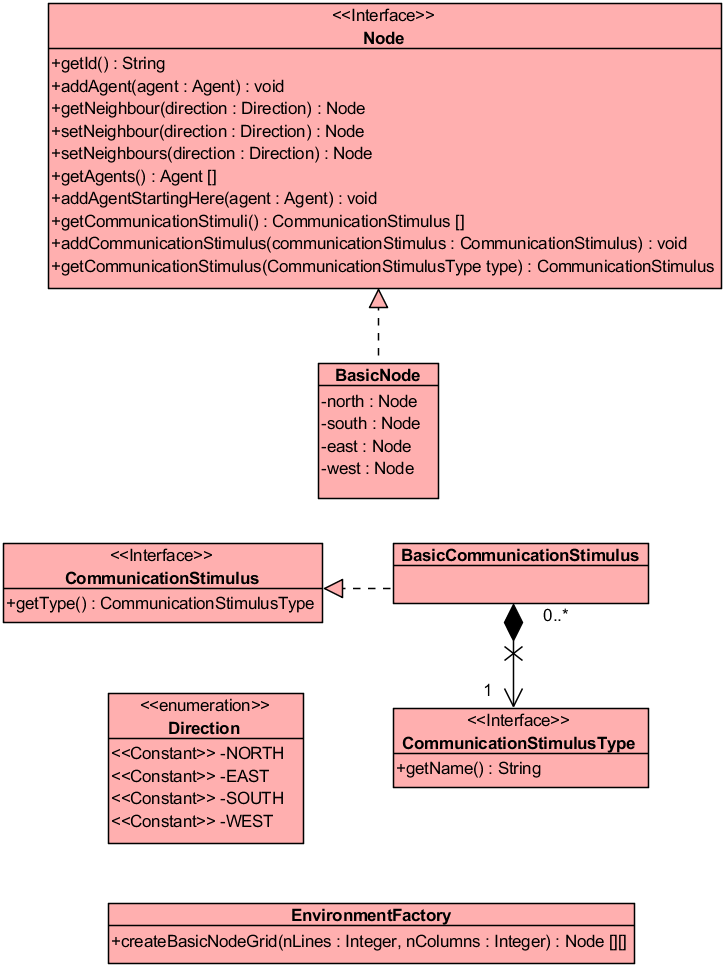
\includegraphics[width=1.0\linewidth]{gfx/uml-env-package.png}
  \caption{Generic model of environment package}
  \label{fig:gen-env-package}
\end{figure}

\section {Agents}
\label{sec:agents}

To enable the agents defined by the model to enjoy the properties that define agents in general it is critical that they have their own lifecycle, and the most flexible way to achieve that is if each agent is run in an isolated thread in one of the available CPUs of the machine running the simulation. This is guaranteed by the \emph{AbstractAgent} which implements the \emph{Callable} interface (see section \ref{subsec:threads-task-exec} for more details).  

The abstraction of any agent is the \emph{Agent} interface though. It formalises the basic API that is available to any agent in the model. The most relevant are:

\begin{itemize}
  \item String getId(): Each agent must have an unique identifier string to be used for identification. This method returns it. Note that is up to the user to make sure this string is unique.
  
  \item AgentType getAgentType(): Returns the type associated with the agent.
  
  \item void setCurrentNode(Node): Places the agent in a specific node of the environment.
\end{itemize}

There are another methods that are related with tracking the nodes the agent has been in the environment during the simulation, more information on these methods can be found in the appendix \ref{chapter:model-code}.

The \emph{AbstractAgent} is the base abstract implementation of the \emph{Agent} interface. It implements all the public methods declared by the interface, plus declares the implementation of the \emph{Callable} interface, returning the type \emph{Void}, which is a convention to tell the compiler that no value is expected to be returned. By being abstract and declaring the implementation of \emph{Callable}, the class effectively forces any concrete specialisation class to implement the methods that define a task in Java, therefore allowing any agent to be executed in an isolated thread.

\subsection{Task Agents}

The smallest unit of work in the computational model is a task, and they are the means to agents to get things done. Please note that this task is different from a Java task discussed in section \ref{subsec:threads-task-exec}. 

In order to enable agents to execute tasks the concrete specialisation of the \emph{AbstractAgent} class, the \emph{TaskAgent} class has a synchronised field called \emph{currentTask} that contains a reference to the task that the agent is executing at the moment. The second difference from the super class, is that task agents have a different \emph{type} associated to them, a \emph{TaskAgentType}, this is important because it is in the \emph{TaskAgentType} that the tasks that an agent is capable of executing are defined, see section \ref{sec:taskagentype} for more details.

\subsection{Agent Types}
\label{sec:agent-types}

In nature individuals use different ways to differentiate themselves from other individuals, in the proposed computational model each agent belongs to a specific type, something that define them as a class. The \emph{AgentType} interface formalises the most basic abstraction of a type of agents.  It has only one method:
\begin{itemize}
  \item String getName(): Returns the name of that type, must be unique.
\end{itemize}
As in the previous cases, the interface does not have any mechanism to make sure a type has a unique name, it is up to de user to make sure that is the case.

An implementation of \emph{AgentType} provides the means for agents to distinguish themselves if necessary, one agent can check another agent’s type when they are in the same node, this is very important, because one agent can react differently if it comes across another agent of the same type or if it encounters an agent that might impose some sort of danger.

In the sake of performance, agent types must implement the Singleton Pattern, which guarantees only one object instance of a type only.\cite{bloch2008effective} If agent types were not to be singletons, every time a new agent is instanced a new agent type and the other objects that compose it, like tasks, are going to be created as well, consuming large amounts of memory. 

\subsubsection{The TaskAgentType type}
\label{sec:taskagentype}

The \emph{TaskAgent} interface is simple and has only one method:

\begin{itemize}
  \item List<Task> getTasks(): Returns a list of tasks that the agents of this type are able to execute.
\end{itemize}

The enumeration \emph{BasicTaskAgentType} is a reference implementation of the interface. Agents of that type are able to execute only one task, \emph{WandererTask}, see section \ref{sec:wanderer-task} for more details on the task.

\subsection{The Ant Interface}

The ant implementation of the model starts from the \emph{Ant} interface. It declares the public API for any agent that is an ant. The most relevant methods are: 

\begin{itemize}
  \item Direction getMovingDirection(): Returns what direction the ant is moving in relation to the environment grid.
  \item void incrementStimulusIntensity(ChemicalStimulusType): Lay pheromone onto the current node that the agent is at.
  \item double collectFood(Agent, double): Tries to collect the specified amount of food from the food source specified as parameter, returns the amount of food that the agent was able to collect.
  \item Boolean isCaringFood(): Returns true if the agent is caring food, false otherwise.
  \item FoodSourceAgent findFoodSource(): Checks if any agent in the current node is a food source, if any is found it is returned otherwise \emph{null} is returned.
  \item void invertDirection(): Inverts the direction the agent is traveling, for example, if the agent is traveling East, after this method is called the agent’s moving direction will be West. See section XXX for more details.
  \item void depositFood(AntNestAgent): Deposit the food the agent is caring into the nest passed as parameter.
\end{itemize}

For the full API and more detail explanations of all the methods, please see section XXX.

\subsection{Ant Agents}
\label{sec:pheromone-deposit}

The \emph{AntAgent} class offer an implementation of the \emph{Ant} interface. Mostly important it has three private methods that are used by \emph{incrementStimulusIntensity (ChemicalCommStimulusType)} for laying pheromone onto the environment. As seen on section \ref{subsec:chemical-stimulus} chemical communication stimulus types have a propriety called \emph{radius} that defines the reach of that particular stimulus around the node where it was deposited, these three methods use this information when depositing pheromone. The intensity of the stimulus decreases as the distance from the node where the agent is at increases according to the following: 

\begin{equation}
intensity_{new} =  intensity_{current} + increase * (1 / distance)
\end{equation}

Figure \ref{fig:distanse-vs-inc} shows how the intensity of the deposited amount of chemical stimulus varies according to the distance to the node the agent is executing the increment. The amount of stimulus that each agent increments is defined by the agent type, see section \ref{sec:agent-types} for a detailed explanation.

\begin{figure}[H]
  \centering
  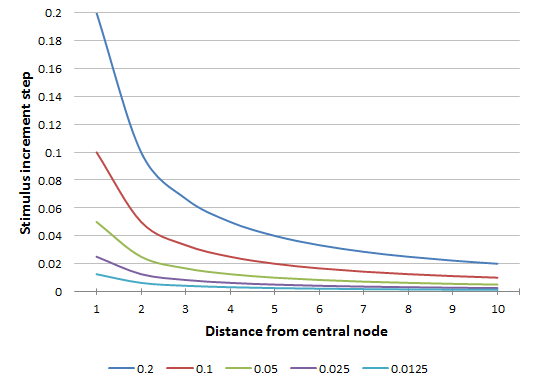
\includegraphics[width=0.5\linewidth]{gfx/distance-vs-increment.png}
  \caption{Variation of increment according to distance to central node}
  \label{fig:distanse-vs-inc}
\end{figure}

Figure \ref{fig:intensity-example} illustrates how the pheromone is laid depending on the radius of the stimulus. The strong the increment is the brighter the red. Each node is represented by a single square. In the image three different radius are demonstrated, form left to right we have 2, 4 and 5 respectively. It is clear that he increment falls as the distance from the central node gets bigger.

\begin{figure}[H]
  \centering
  
\includegraphics[width=0.5\linewidth]{gfx/intensity-example.png}
  \caption{Pheromone deposit for stimulus with different radius sizes}
  \label{fig:intensity-example}
\end{figure}

\subsection{Ant types}

The interface \emph{AntType} and its implementations are used to represent any specific type of ant in the computational model. The interface declares the following methods:

\begin{itemize}

  \item void execute(Agent): Method executed when the agent is executed by the thread pool.
  \item double getStimulusIncrement(String): Returns the amount of stimulus the agent is able to lay.
  \item int getMemorySize(): The number nodes the agent can remember it has been.
  \item double getAmountOfFoodCapableToCollect(): Returns the amount of food the agent is capable of caring 

\end{itemize}

(((need to discuss the way the memory is implemented)))

By far the most important method in the list is \emph{void execute(Agent)}, because this method is the method that defines the agent's behaviour. It is in this method the agent can analyse the environment state around it and decide which tasks to execute.

As seen, different type of ants are able to deposit different types of pheromone and in different quantities. So every type of ant has a map that tells by name, what is the increment for each stimulus the ant is able to deposit. the method \emph{double getStimulusIncrement(String)} is used to query these amounts.

\subsubsection{WorkerType}

The enumeration \emph{WorkerType} defines the type of ant that represent workers in a colony. The type is capable of executing three tasks, \emph{ForageTask}, \emph{FindHomeTask} and \emph{FindAndHideInNestTask}. Ants of this type are sensitive can lay \emph{ForageStimulusType} and low quantities of \emph{WarningStimulusType}. 

The goal of this type of ant is to explore the environment, find food,  collect as much as possible and take it back to the nest. Figure \ref{fig:worker-type} fully describes the algorithm implemented by the \emph{WorkerType}.

\begin{figure}[H]
  \centering
  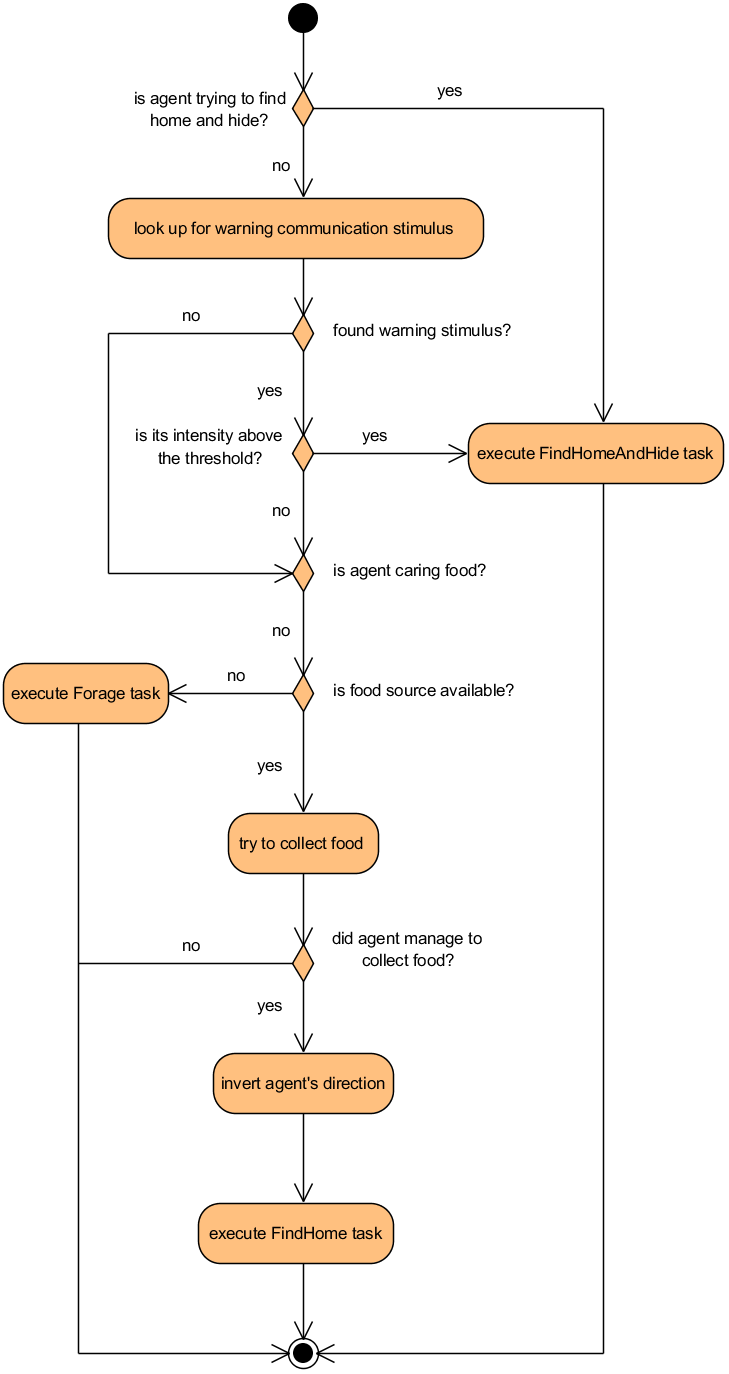
\includegraphics[width=0.8\linewidth]{gfx/uml-worker-type.png}
  \caption{Worker Type ant algorithm}
  \label{fig:worker-type}
\end{figure}

\subsubsection{Ant Nests}

The enumeration \emph{AntNestType} declares a type of agent that represents an ant nest. It implements the base \emph{AgentType} interface, so as one would expect, agents of this types are not able to execute tasks.

The class \emph{AntNestAgent} is an specialisation of \emph{AbstractAgent}, it has an extra synchronised field that works as a counter of how much food is available in the nest, \emph{amountOfFoodHeld}. It also declares a public method called \emph{void addPortionOfFood(AntAgent, double)} which allows ants to deposit food in the nest.

\subsection{Agents Package}

\begin{figure}[H]
  \centering
  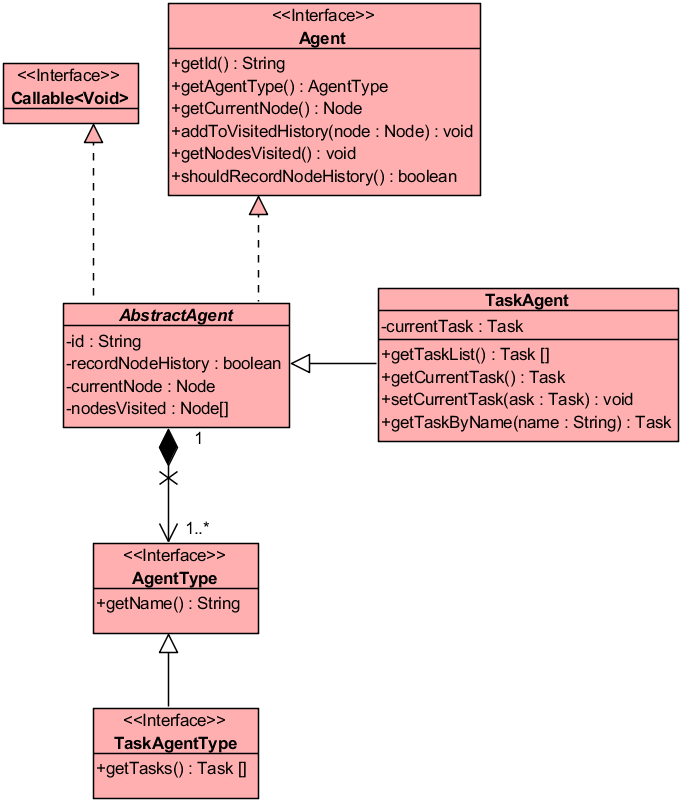
\includegraphics[width=1.0\linewidth]{gfx/uml-agent-package.png}
  \caption{Generic model of the agent package}
  \label{fig:gen-agent-package}
\end{figure}


\section {Tasks}

Tasks are a unit of specialised work. They are the means to agents to do something they need to do. Different type of agents can share the same task, but it is up to each of them how to use it.

The \emph{Task} interface formalises two methods:

\begin{itemize}
  \item String getName(): Returns the unique name that identifies the task.
  
  \item void execute(Agent): Runs the task algorithm for the agent used as parameter.
\end{itemize}

Tasks are a convenient way to process unit of work that are isolated one from another and done by more than one type of agent. The \emph{void execute(Agent)} method contains the actions that the task is to perform, the agent that is requesting the task execution is passed as a parameter so the task is able to access the agent's context, such as neighbours and communication stimuli. The \emph{AbstractTask} class provides the base implementation for concrete tasks.

\subsection{Wanderer Task}
\label{sec:wanderer-task}

This task is a simple task that agents can use when they are exploring the environment, it causes the agent to move from the current node to one of the available neighbours. It selects which neighbour to move to completely at random.

In the case of ants, for example, they use this task when looking for a new source of food or when they reach one of the environment boundaries and need to switch their moving direction.

\subsection{Ant Tasks}
\label{sec:ant-tasks}

Ants execute tasks that implement the \emph{AntTask} interface. For the list of methods of the interface, please see XXX.

\subsubsection{Forage Task}
\label{task:forage}

The \emph{ForageTask} is also used by agents to find food sources and collect food. Differently from the \emph{WandererTask}, it does not pick a node to move to at random, it follows the forage chemical stimulus trail.

Although the pheromone trail is the most important part when the agents are deciding where to go next, another effects should be considered, for instance an agent could be taken away from the trail by the wind or if some information, like chemical landmarks, that the ants use to locate themselves is modified, should somehow be considered. Tt virtually impossible to model all this cases though, more, it would be wrong to try to model all the possible interferences in the colony.

So, the agents present a stochastic behaviour as far as moving through the space is concerned. So the process of choosing the node to move to consists of: 

\begin{enumerate}
  \item Each neighbour node is associated with a weight.
  \item The weights are multiplied by the actual pheromone trail found in  each of the neighbour nodes.
  \item The results of each multiplication in the previous step are summed up to a total.
  \item Each multiplication of step 2 is divided by the total, in order to find their ratio.
  \item A Monte Carlo (((cite))) like selection on the neighbour nodes is executed using these rates.
\end{enumerate}

\begin{figure}[H]
  \centering
  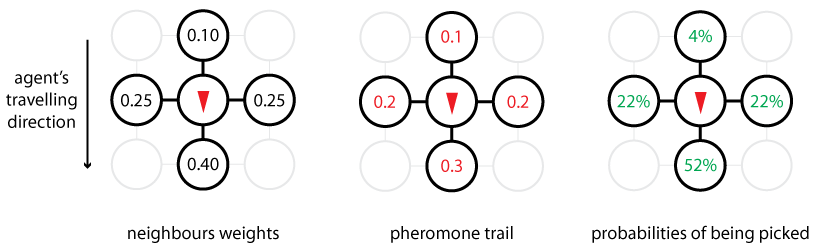
\includegraphics[width=0.9\linewidth]{gfx/choosing-next-node.png}
  \caption{Elements used to select next node to move to}
  \label{fig:choosing-next-node}
\end{figure}

Figure \ref{fig:choosing-next-node} illustrates these steps. It is important to understand that when applying the weights to the neighbours the task uses the agent as reference not the grid. As an example, if we imagine a agent with the moving direction set to East in relation to the grid, so the east neighbour from the node that the agent sits is pointing to the north direction of the agent. Figure \ref{fig:position-reference} illustrates that.

\begin{figure}[H]
  \centering
  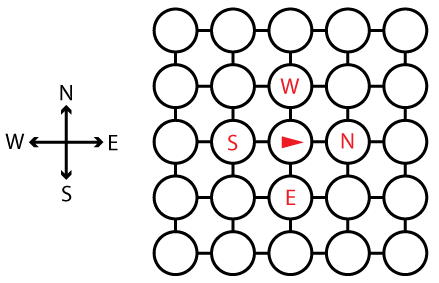
\includegraphics[width=0.5\linewidth]{gfx/reference.png}
  \caption{Reference of directions}
  \label{fig:position-reference}
\end{figure}

It is necessary to know what direction the agent is travelling to and perform this transformation between the grid direction reference to the agent's in order to apply the right selection weights to the neighbour nodes.

This method of selection is implemented by the utility class \emph{AntTaskUtil} and is used in other tasks as well. The method is flexible enough to allow tasks to set their own weights for the neighbour nodes and ask any type of chemical stimulus to be used in the calculation.

Figure \ref{fig:forage-activity} is the active diagram of the algorithm implemented by the \emph{void execute(Agent)} method of the \emph{ForageTask}.

\begin{figure}[H]
  \centering
  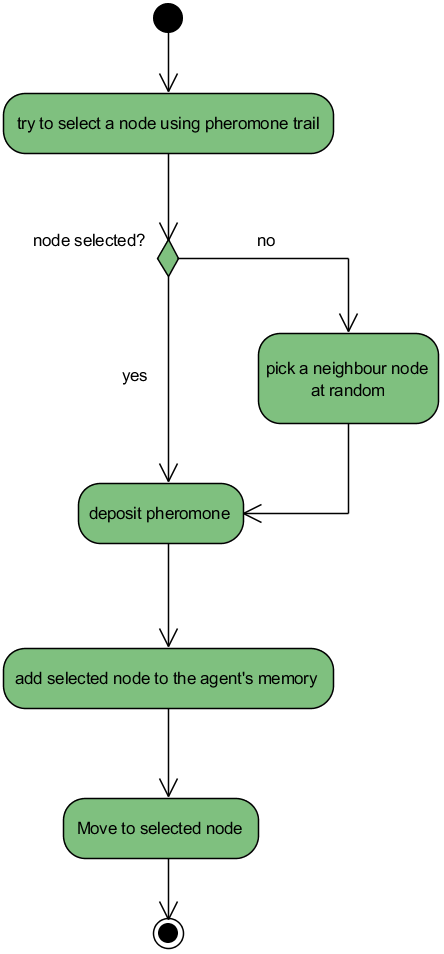
\includegraphics[width=0.6\linewidth]{gfx/uml-act-forage.png}
  \caption{Forage task execution activity diagram}
  \label{fig:forage-activity}
\end{figure}

\subsubsection{Find Home Task}
\label{task:find-home}

The \emph{FindHomeTask} is useful for ants that have collected food and need to deposit it in their nest. It uses the same procedure that \emph{ForageTask} to select which node to move next. The biggest difference is that it tries to use the agent's memory before following the specified pheromone trail. The task's algorithm is illustrated in Figure \ref{fig:find-home-act}.

\begin{figure}[H]
  \centering
  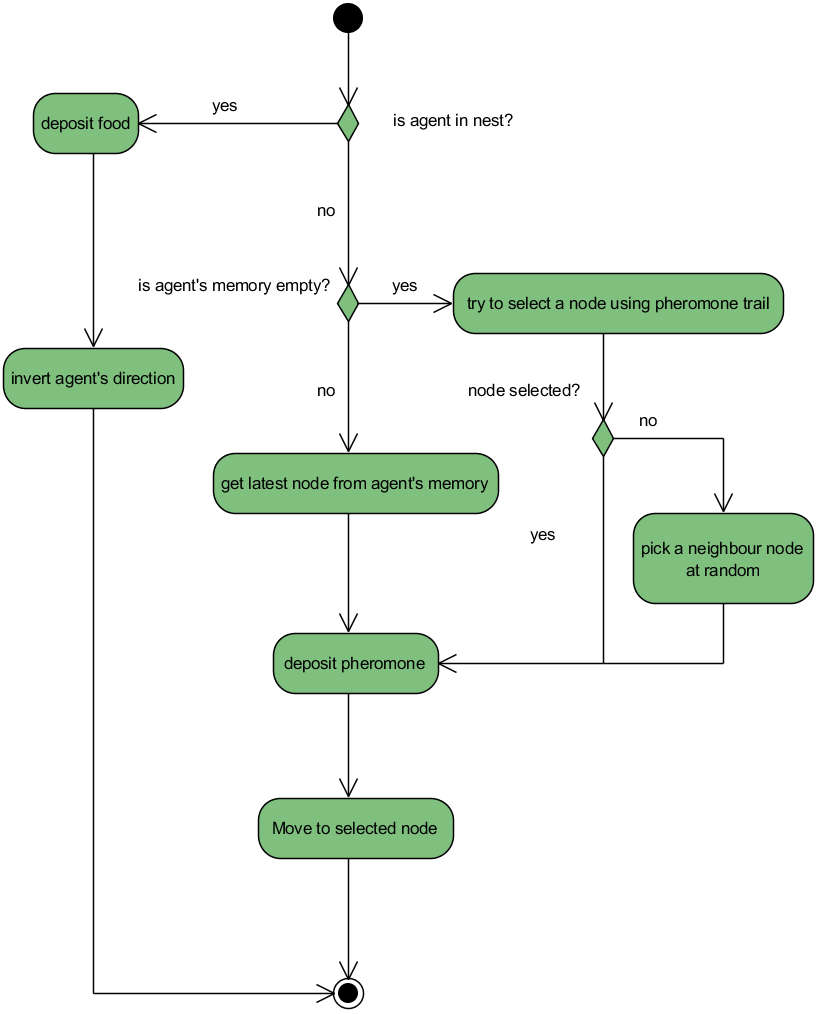
\includegraphics[width=0.9\linewidth]{gfx/uml-act-home.png}
  \caption{Find home task execution activity diagram}
  \label{fig:find-home-act}
\end{figure}

\subsubsection{Find Home And Hide}
\label{task:find-home-hide}

The \emph{FindHomeAndHideTask} is very similar to \emph{FindHomeTask} the only difference is that if the agent is in a node that contains a nest the task does not try to do anything else, it leaves the agent there. 

is useful for ants that have collected food and need to deposit it in their nest. It uses the same procedure that \emph{ForageTask} to select which node to move next. The biggest difference is that it tries to use the agent's memory before following the specified pheromone trail. The task's algorithm is illustrated in Figure \ref{fig:find-home-hide-act}.

\begin{figure}[H]
  \centering
  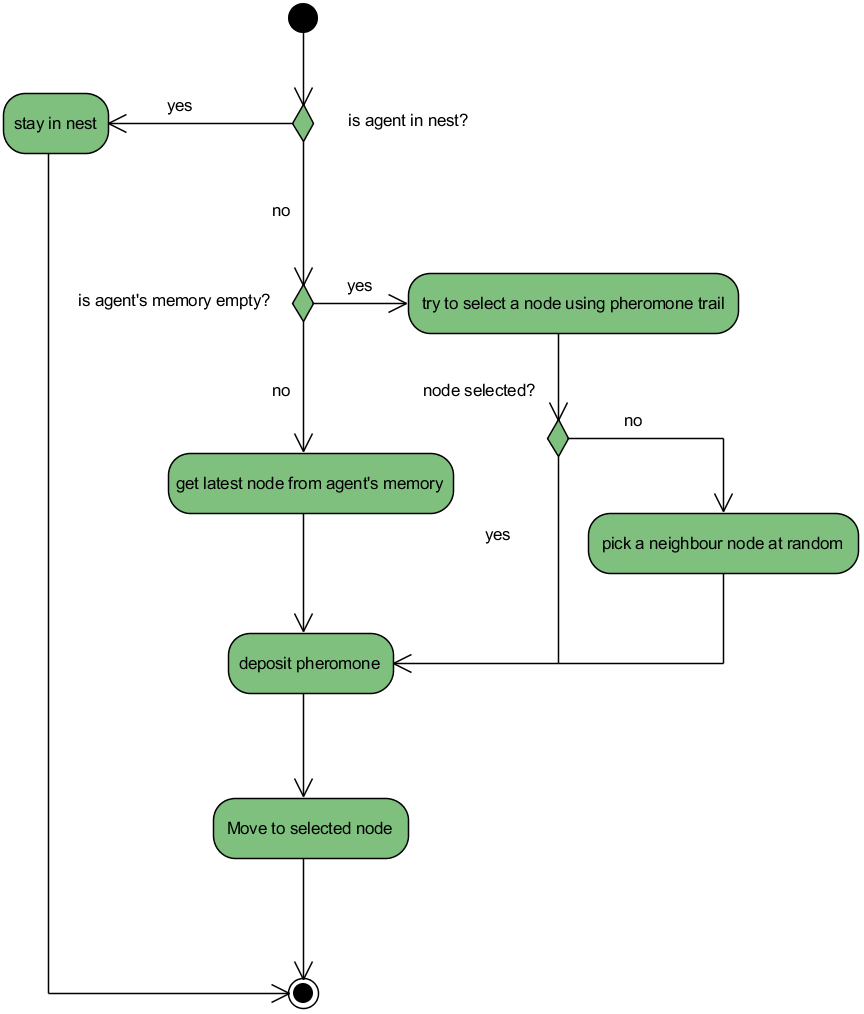
\includegraphics[width=0.8\linewidth]{gfx/uml-act-home-hide.png}
  \caption{Find home and hide task execution activity diagram}
  \label{fig:find-home-hide-act}
\end{figure}

\section {Generic Computational Model Diagram}

\begin{figure}[H]
  \centering
  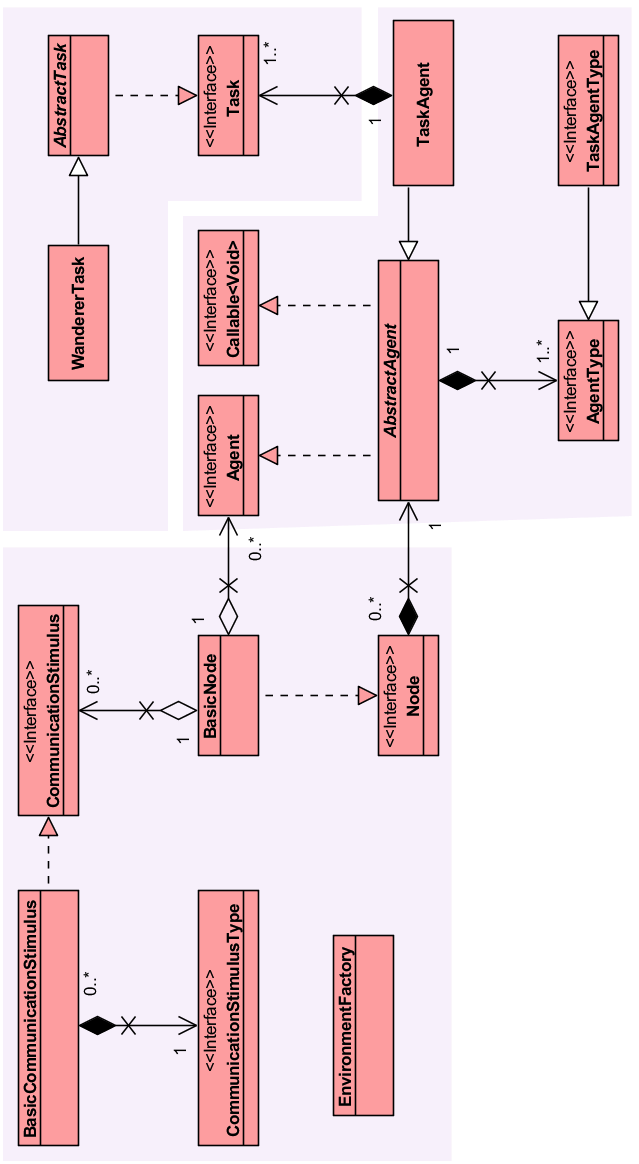
\includegraphics[width=0.7\linewidth]{gfx/uml-generic-overview.png}
  \caption{Generic Computational Model}
  \label{fig:generic-model}
\end{figure}

\cleardoublepage % Empty page before the start of the next part

%------------------------------------------------

\ctparttext{In this part of the report three experiments are proposed and executed. The results observed are discussed. At the end some possible improvements to the model and possible experiments are proposed.}

\part{Experiments And Observations} % Second part of the thesis

\chapter{Experiments And Observations}
\label{ch:experiments-and-observations}

\section{Simulations and data collection}
\label{sec:running-sim}

The computational model does not formalise any resources to be used to create and run simulations, neither the model formalise any way to collect data from the simulations.

JUnit is the reference unit test framework for Java, and the basic implementation of the proposed computational model is tested against more than 20 unit tests. However, unit tests also provide the perfect environment to run simulations. If resources such as initial node grid, initial pheromone concentrations and agents are going to be the same for more than one simulation, one can take advantage of test \emph{fixture} with the \emph{@Before} annotation to initialise these objects without repeating code. One could could create a class for each simulation with a \emph{Main} method also, however it is more convenient to use the test framework.

Another critical aspect of the simulations is data collection. The model does not describe how data can be acquired during and after the simulation. For the simulations run for this paper logging was used for this intend. Log4j is a thread-safe logging service maintained by the Apache foundation and it was used throughout the implementation and the simulations. In most of the simulations the logger was setup to write into files that are processed after the simulation is finished. Also, it is possible to configure the logger service to write on the console, so information on the agents can be easily visualised during the execution of the simulations.

\section{Pheromone Concentration Sensibility}

Due to the model of node selection agents are sensitive to the pheromone concentration presented by the environment around them. This happens because the probability of choosing a neighbour node swings form $0$ to a $100$ percent very swiftly, causing the agents to get trapped.

This experiment investigates how different initial pheromone concentrations in the environment and the amount of pheromone each agent is capable of depositing in each interaction affect the agents navigation through the space. It also has objective to determine what values of these two parameters are acceptable to use in the other experiments.

Firstly, let's examine the case when all the nodes of the environment are created with no initial concentration of \emph{Forage} pheromone (Figure \ref{fig:initial-a}). When the agent is deciding which node it is going to make the first move to, all neighbours have the same probability of being picked, because of the $0$ of pheromone concentration (Figure \ref{fig:initial-b}). So as it was programmed to, the agent picks one node at random. But before moving to the next node it lays a bit of pheromone, suppose the concentration deposited is $0.1$. When the move is done, the environment around the agent should look like the one pictured in Figure \ref{fig:initial-c}.

\begin{figure}[H]
\myfloatalign
\subfloat[Initial environment]
{\label{fig:initial-a}
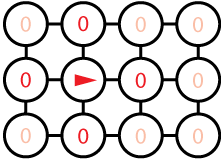
\includegraphics[width=.3\linewidth]{gfx/initial-01}} \quad
\subfloat[Initial probabilities]
{\label{fig:initial-b}
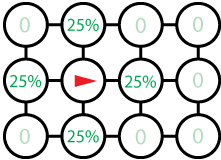
\includegraphics[width=.3\linewidth]{gfx/initial-02}} \\
\subfloat[Environment after move 1]
{\label{fig:initial-c}
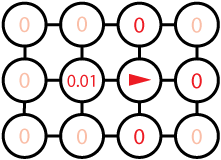
\includegraphics[width=.3\linewidth]{gfx/initial-03}} \quad
\subfloat[Probabilities after move 1]
{\label{fig:initial-d}
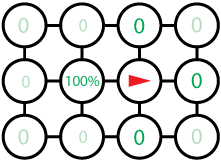
\includegraphics[width=.3\linewidth]{gfx/initial-04}} \\
\subfloat[Environment after move 2]
{\label{fig:initial-e}
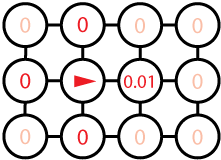
\includegraphics[width=.3\linewidth]{gfx/initial-05}} \quad
\subfloat[Probabilities after move 2]
{\label{fig:initial-f}
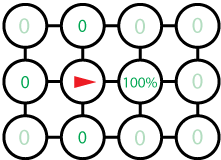
\includegraphics[width=.3\linewidth]{gfx/initial-06}}

\caption{Affect of initial pheromone concentration at zero}\label{fig:initial}
\end{figure}

Now it is time for the agent to move again. Firstly the agent reads the pheromone intensity in each of the neighbour nodes, after it computes where it is more likely to move. For all the nodes around the agent apart from the one it has just moved from have $0$ pheromone intensity in them, the agent is certain to move back to the previous node (Figure \ref{fig:initial-d}). Before completing the move, it lays pheromone in the current node. When the agent is back to the node it first started from, the scenario repeats and it becomes a cycle. The agent go back and forth, trapped in these two nodes forever, with no changes to explore the environment further. 

It is clear that the environment cannot be initialised with no \emph{Forage} pheromone in its nodes. The question that arises from this is: Is there any pair of values for these two parameters that will allow the agents to navigate in an acceptable fashion?

To answer this question, the experiment was setup with the following configuration:

\begin{table}[H]
\myfloatalign
\begin{tabularx}{\textwidth}{Xll} \toprule
\tableheadline{Property} & \tableheadline{Value} \\ \midrule
Number of lines & 500 \\
Number of columns & 500 \\
Total number of nodes &  250,000 \\
\midrule
Duration of each simulation & 10 s \\
Number of agents & 50 \\
Agent Type & WorkerType \\
Task executed & ForageTask \\
Agent sleep time & 5 ms \\
\bottomrule
\end{tabularx}
\caption{Experiment setup for investigation of initial pheromone concentration}  
\label{tab:setup-1}
\end{table}

In Table \ref{tab:setup-1} the property \emph{Agent sleep time} means how long the agent waits after a task is executed to choose another task to run. This is necessary to slow down agents (in this case the threads that are running the agent), otherwise they would cover the entire space in this 10 seconds only by the fact that they can do it very fast not because they are actively foraging.

The initial pheromone concentration and the amount of pheromone deposited in each interaction by the agents were varied from $0.001$ to $0.04$ in $5$ steps. Each of the possible pair of values for the two parameters has been simulated:

\begin{table}[H]
\myfloatalign
\begin{tabularx}{\textwidth}{XXXXX} \toprule
\tableheadline{1} & \tableheadline{2} & \tableheadline{3} & \tableheadline{4} & \tableheadline{5} \\ \midrule
0.001, 0.001 & 0.001, 0.005 & 0.001, 0.01 & 0.001, 0.02 & 0.001, 0.04 \\
0.005, 0.001 & 0.005, 0.005 & 0.005, 0.01 & 0.005, 0.02 & 0.005, 0.04 \\
0.01, 0.001 & 0.01, 0.005 & 0.01, 0.01 & 0.01, 0.02 & 0.01, 0.04 \\
0.02, 0.001 & 0.02, 0.005 & 0.02, 0.01 & 0.02, 0.02 & 0.02, 0.04 \\
0.04, 0.001 & 0.04, 0.005 & 0.04, 0.01 & 0.04, 0.02 & 0.04, 0.04 \\
\bottomrule
\end{tabularx}
\caption{Variations for initial concentration and amount of pheromone deposited by agents}  
\label{tab:setup-2}
\end{table}

In each case, the colony containing $50$ agents is created at the north of the environment, horizontally centred. The agents execute the \emph{ForageTask} since their creation, they do not analyse any contextual parameters such as other agents, they only try to move through the space using the rules defined by the task.

In order to compare how each possible value pairs in Table \ref{tab:setup-2} affect the resulting navigation of the agents, two samples of  the pheromone trail left by the agents are analysed. The first one is from close to the nest that will enable us to check how is the agents' response to the initial pheromone concentration shortly they have left the nest. The second sample is taken further ahead in the environment, far from the nest. This sample is a good way to test how the agents' own deposit of pheromone will affect the system behaviour, Figure \ref{fig:initial-sample} illustrates how and where the samples are made.

\begin{figure}[H]
  \centering
  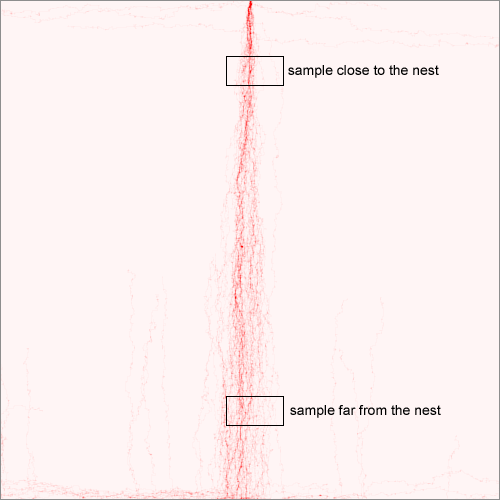
\includegraphics[width=0.5\linewidth]{gfx/initial-sample.png}
  \caption{How the two samples of the environment is made}
  \label{fig:initial-sample}
\end{figure}

Figures \ref{fig:initial-var-close} and \ref{fig:initial-var-far} show the resulting sampling for all possible combination for the initial pheromone concentration and the amount of pheromone deposited by each agent in each interaction.

\begin{figure}[H]
  \centering
  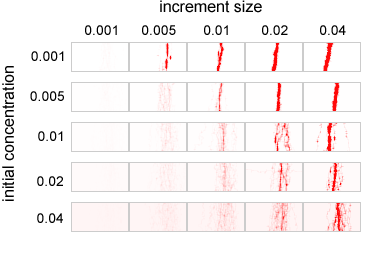
\includegraphics[width=0.6\linewidth]{gfx/initial-variations-close.png}
  \caption{Resulting pheromone trail close to the nest}
  \label{fig:initial-var-close}
\end{figure}


\begin{figure}[H]
  \centering
  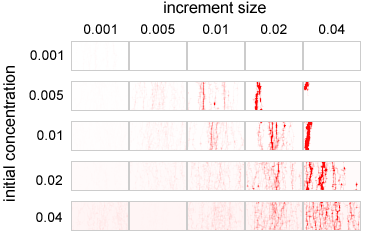
\includegraphics[width=0.6\linewidth]{gfx/initial-variations-far.png}
  \caption{Resulting pheromone trail far from the nest}
  \label{fig:initial-var-far}
\end{figure}

The trails left by the colonies can be compared in relation on how strong they are, how the agents are able to 'scape' them to explore the environment and how it shaped when agents get further from the nest.

Starting from $0.001$ as the amount of pheromone to be deposited by agents in each interaction; it is possible to observe from the figures that two very contrasting behaviours emerge, firstly because the environment has so little pheromone and the update is so small, they weight assigned to each of the neighbour nodes count considerably more than the pheromone deposited by the agents, so the agents end up very dispersed, thus no chemical trail is formed at all. This phenomena is actually seen in many other combination of the parameters, all the cases when the update is $0.001$ in fact. 

When the amount of pheromone deposited by the agents is increased the behaviour of the colony could not be more different than what was seen previously. The agents switch from exploring a large area to be 'trapped' into the pheromone trail. This impedes the agents of exploring the space, what is not desirable for any colony. This behaviour is also seen in other values for the parameters. What seems to be the rule is that if the update is considerable larger than the concentration of pheromone in the environment the agents will start to create a 'bubble' of high pheromone concentration and as consequence they are very unlikely to move to any node outside this area.

It rises the question, why does it happen? The answer is similar to one of the problem in initialising the environment with no pheromone at all. In this case, the critical point is the rate between the initial concentration and the amount deposited by the agents in each interaction.

\begin{figure}[H]
\myfloatalign
\subfloat[]
{\label{fig:update-a}
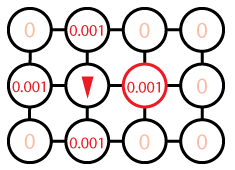
\includegraphics[width=.2\linewidth]{gfx/update-01}} \quad
\subfloat[]
{\label{fig:update-b}
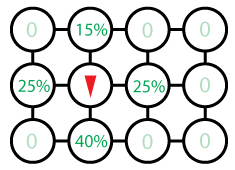
\includegraphics[width=.2\linewidth]{gfx/update-02}} \\
\subfloat[]
{\label{fig:update-c}
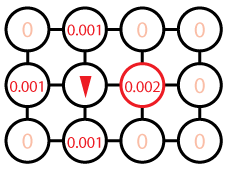
\includegraphics[width=.2\linewidth]{gfx/update-03}} \quad
\subfloat[]
{\label{fig:update-d}
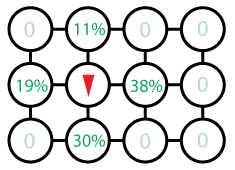
\includegraphics[width=.2\linewidth]{gfx/update-04}} \\
\subfloat[]
{\label{fig:update-e}
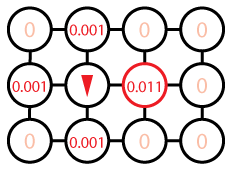
\includegraphics[width=.2\linewidth]{gfx/update-05}} \quad
\subfloat[]
{\label{fig:update-f}
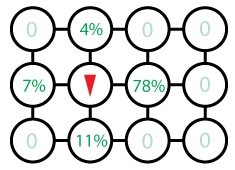
\includegraphics[width=.2\linewidth]{gfx/update-06}}

\caption{Shift of probability depending on agent update}\label{fig:update}
\end{figure}

Figure \ref{fig:update} illustrates how swiftly the probabilities can change depending on the amount of pheromone deposited in the node by agents. The node in red in the picture represents a node that has been updated previously by another agent. In the first scenario (Figure \ref{fig:update-c}) the update was $0.001$, in the second (Figure \ref{fig:update-e}) the pheromone deposited was $0.01$. The probability of the node in red being picked up to be the next node the agent will move to more than doubled. (Figure \ref{fig:update-d} and Figure \ref{fig:update-f}).

Further investigation revealed that the probability of selection increases in a logarithmic-like curve. Figure \ref{fig:prob-inc} shows how the increase in probability progress when the amount of pheromone deposited by the agents increases by multiples of the initial concentration in the environment.

\begin{figure}[H]
  \centering
  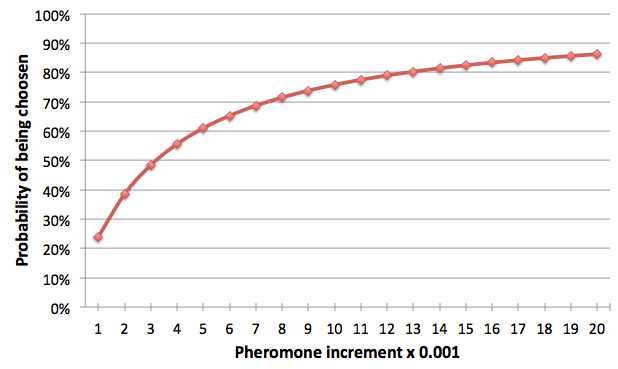
\includegraphics[width=0.6\linewidth]{gfx/probability-increase.png}
  \caption[Selection probability increasing]{Increase of probability selection according to the increase of the deposit increment}
  \label{fig:prob-inc}
\end{figure}

It is very tempting to conclude that if the right ratio between the initial pheromone concentration and the increment step used by the agents is found the, problems of the lack of trail formation and the agent confinement in the trail will be solved. However from figures \ref{fig:initial-var-close} and \ref{fig:initial-var-far} it is observed that the same ratio (initial concentration/increase step) present different results for different values. In the case $0.001/0.001$ no trail is formed at all, for $0.01/0.01$ a solid trail is formed. 

The experimental results are that the initial pheromone concentration should not be too low that avoid trail formation or saturation. It has to be an intermediate value that allows the agents to converge to a specific path, generating the trail, but not too fast, allowing the agents to explore other parts of the environment as well. As far as the update step goes, it also needs to be an intermediate value, so it starts actually being part of the node selection process but not big enough to quickly saturate the pheromone trail.

\begin{figure}[H]
\myfloatalign
\subfloat[]
{\label{fig:trail-a}

\includegraphics[width=.1\linewidth]{gfx/trail-001}} \quad
\subfloat[]
{\label{fig:trail-b}
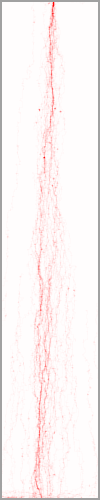
\includegraphics[width=.1\linewidth]{gfx/trail-01}} \quad
\subfloat[]
{\label{fig:trail-c}
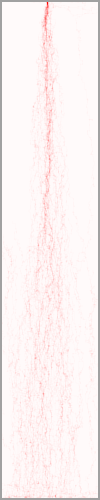
\includegraphics[width=.1\linewidth]{gfx/trail-0201}} \quad
\subfloat[]
{\label{fig:trail-d}
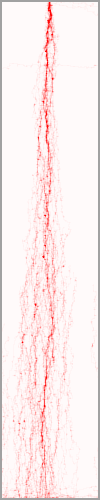
\includegraphics[width=.1\linewidth]{gfx/trail-0202}} \quad
\subfloat[]
{\label{fig:trail-e}
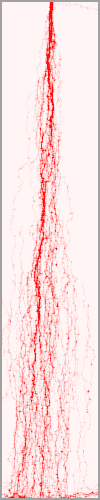
\includegraphics[width=.1\linewidth]{gfx/trail-0404}} \quad

\caption[Example of complete pheromone trails]{Complete trail pheromone trails left by simulation using 0.001,0.04 (a), 0.01,0.01 (b), 0.02,0.01 (c), 0.02,0.02 (d) and 0.4,04 (e) for initial pheromone concentration and update step respectively}
\label{fig:trails}
\end{figure}

One can conclude from this analysis pair $0.01/0.01$ (Figure \ref{fig:trail-b}) for the initial pheromone concentration and increment step present the best results. It allows pheromone trail to \emph{emerge as a result of the agents' interactions with the environment}. It could also be argued that another pairs such $0.01/0.02$ and $0.02/0.02$ set the right conditions for agent navigation. However, in this experiment the agents are executing the \emph{ForageTask} without actually collecting food, to no agent tries to deposit food in the nest and start foraging again - the trail is not reinforced. Taking that in consideration the other pairs tested could also be considered to lead to a premature saturation of the trail, which is the case of $0.02/0.02$.

The pair $0.01/0.01$ also proved to be less sensitive to the number of agents used in this and the other experiments.

\section{Forage Radius Investigation}
\label{sec:forage-radius-inv}

This experiment investigates the affect of the radius variation of the \emph{Forage} chemical stimulus (section \ref{subsec:forage-stimulus}) on the capacity of the colony to collect food. Four values for the stimulus' radius were tried - $0$, $1$, $2$. The experiment was setup as follows:

\begin{table}[H]
\myfloatalign
\begin{tabularx}{\textwidth}{Xll} \toprule
\tableheadline{Property} & \tableheadline{Value} \\ \midrule
Number of lines & 500 \\
Number of columns & 500 \\
Total number of nodes &  250,000 \\
Initial grid pheromone intensity & 0.01 \\
\midrule
Pheromone radius variations & 0, 1, 2 \\
Duration of each simulation & 30 s \\
Number of agents & 50 \\
Agent Type & WorkerType \\
Pheromone increment step & 0.01 \\
Task executed & ForageTask and FindHome\\
Agent sleep time & 5 ms \\
Pheromone decay frequency & every 3 seconds \\
\bottomrule
\end{tabularx}
\caption{Experiment setup for pheromone radius variation study}  
\label{tab:setup-2}
\end{table}

In this experiment the radius of action of the forage pheromone is varied in order to check the effects in the amount of food the colony is capable of forage. At first one would expect that the increase on the radius of the forage pheromone would have a positive impact on the colony capacity of collecting food as trails that lead to food sources would are reinforced by agents caring food back to the nest and with a wider spread of the pheromone more workers would be fall in these trails. However the data from the simulations show a different picture. The colony collect less and less food as the stimulus' radius increase. Table \ref{tab:radius-results} is a summary of the data collected from the study.

For this experiment a row of food sources was placed far away from the colony. Each source has a total amount of food of $30$. The simulation was run $100$ times for each radius variation. Figure \ref{fig:radius-res} presents part of the middle section (see Figure \ref{fig:radius-full-a}) of the trails created by the agents for the first $20$ simulations for each value used for radius.

\begin{figure}[H]
\myfloatalign
\subfloat[radius = 0]
{\label{fig:radius-res-a}
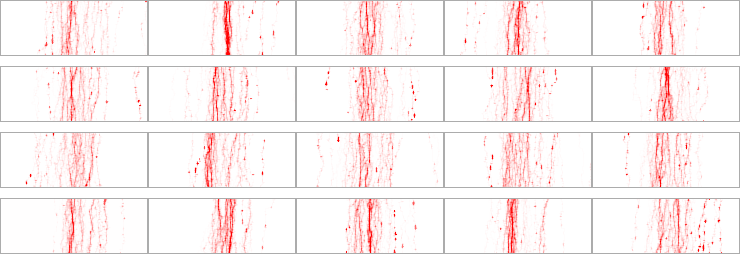
\includegraphics[width=.8\linewidth]{gfx/radius-res-0}} \\
\subfloat[radius = 1]
{\label{fig:radius-res-b}
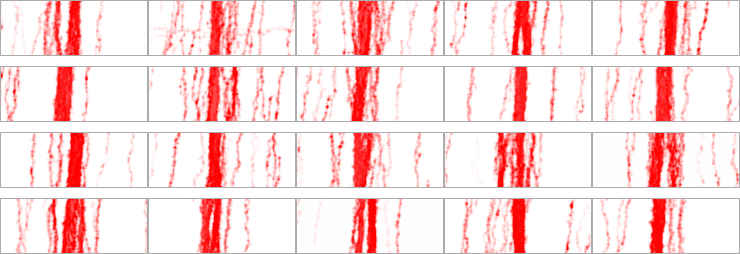
\includegraphics[width=.8\linewidth]{gfx/radius-res-1}} \\
\subfloat[radius = 2]
{\label{fig:radius-res-c}
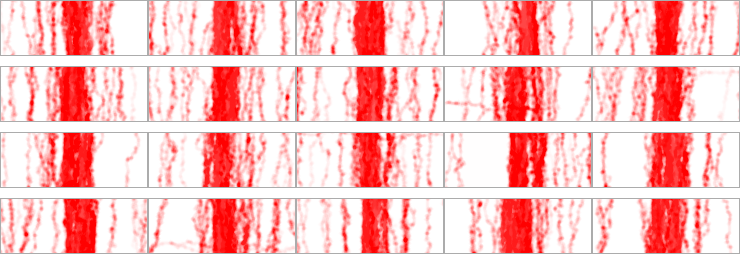
\includegraphics[width=.8\linewidth]{gfx/radius-res-2}} \\

\caption[Visual samples of variation of radius]{20 graphical samples of the results in variating forage stimulus' radius}\label{fig:radius-res}
\end{figure}

\begin{figure}[H]
\myfloatalign
\subfloat[setup]
{\label{fig:radius-full-a}
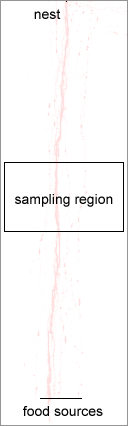
\includegraphics[width=.15\linewidth]{gfx/radius-experiment}} \quad
\subfloat[radius = 0]
{\label{fig:radius-full-b}
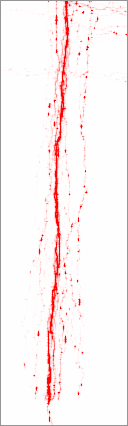
\includegraphics[width=.15\linewidth]{gfx/radius-full-0}} \quad
\subfloat[radius = 1]
{\label{fig:radius-full-c}
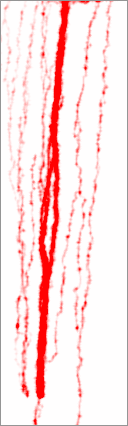
\includegraphics[width=.15\linewidth]{gfx/radius-full-1}} \quad
\subfloat[radius = 2]
{\label{fig:radius-full-d}
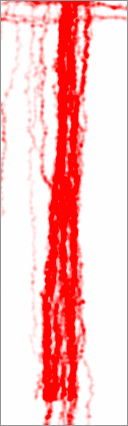
\includegraphics[width=.15\linewidth]{gfx/radius-full-2}}

\caption{Example of trail formation for different radiuses}
\label{fig:radius-full}
\end{figure}

\begin{table}[H]
\myfloatalign
\begin{tabularx}{\textwidth}{Xll} \toprule
\tableheadline{Radius} & \tableheadline{Average of food collected} & \tableheadline{Standard deviation} \\ \midrule
0 & 6.0 & 1.21 \\
1 & 4.9 & 0.72 \\
2 & 3.3 & 0.53 \\

\bottomrule
\end{tabularx}
\caption{Forage radius simulations' outcomes}  
\label{tab:radius-results}
\end{table}

The averages that are presented in the Table \ref{tab:radius-results} was calculated after statistically validating the dataset collected for each radius value, with any outlier sample was removed from the results collected from the simulations. The following pair of equation are used to define a sample point $x_i$ as outlier or not:

\begin{equation}
\begin{cases} 

x_{i} \leq \bar{x} - 2 \times \sigma \\
x_{i} \geq \bar{x} + 2 \times \sigma

\end{cases}
\end{equation}

Where $\bar{x}$ is the average of the resulting dataset for each radius and $\sigma$ is the standard deviation. The data collected proved to be consistent and only few samples were rejected. Figure \ref{fig:radius} shows the samples spread for each radius and their probability density distribution.

\begin{figure}[H]
\myfloatalign
\subfloat[]
{\label{fig:radius-a}
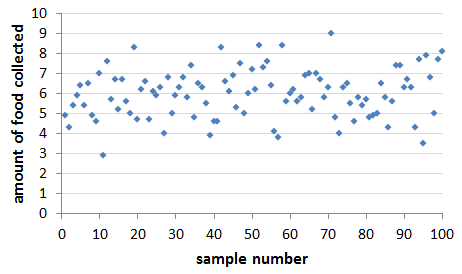
\includegraphics[width=.4\linewidth]{gfx/radius-0}} \quad
\subfloat[]
{\label{fig:radius-b}
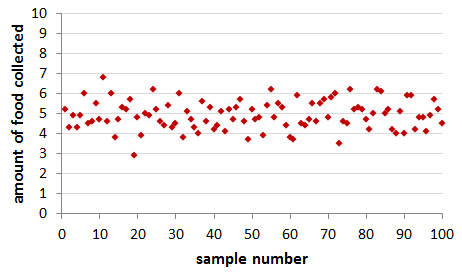
\includegraphics[width=.4\linewidth]{gfx/radius-1}} \\
\subfloat[]
{\label{fig:radius-c}
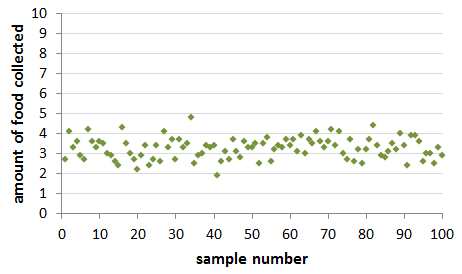
\includegraphics[width=.4\linewidth]{gfx/radius-2}} \quad
\subfloat[]
{\label{fig:radius-d}
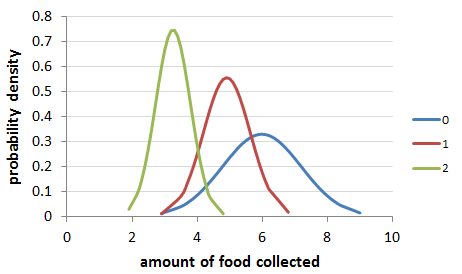
\includegraphics[width=.4\linewidth]{gfx/radius-pdf}}

\caption[Radius variation - samples distributions]{Samples distribution variating the pheromone radius - 0 (a), 1 (b) and 2 (c) - and the samples' probability density distribution (d)}\label{fig:radius}
\end{figure}

Figure \ref{fig:radius} helps to visualise what the standard deviations from Table \ref{tab:radius-results} had already shown - the samples \emph{variance} decreases when the radius increases. The reason for this phenomena is that the bigger the pheromone radius is the lesser agents are probable to 'escape' from the trail, thus they are not able to explore different areas of the environment. For the agents use virtually only the same pheromone trail to forage their outcomes are likely to be very close.  

With a more diversified exploratory reach, agents in the simulations using radius $0$ are likely to have different degrees of success in finding food and taking it back to the nest in each simulation run, justifying the greater variance in the colony outcome.

The study carries raises another question - why does smaller radiuses outperform bigger ones? From Table \ref{tab:radius-results} we can see that the simulations with radius $0$ outperforms the ones with radiuses $1$ and $2$ in $22$ and $82$ percent in average respectively. This occurs due to the formation of trails with large width, leading the agents to move from note to node in almost random fashion. 

Figure \ref{fig:radius-res} illustrates how the pheromone trails widen with the increase of the pheromone radius. It might seem contradictory at first that wider trails do not led to better forage performance, for more ants should be lead to food sources. However due to the model of node selection implemented the agents are too sensitive to the pheromone intensity of the direct neighbours of the node they are currently at, and this is translated to random node selection when agents are trapped in wide pheromone trails. 

\begin{figure}[H]
\myfloatalign
\subfloat[]
{\label{fig:radius-sat-a}
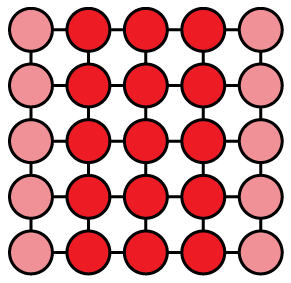
\includegraphics[width=.3\linewidth]{gfx/radius-sat}} \quad
\subfloat[]
{\label{fig:radius-sat-b}
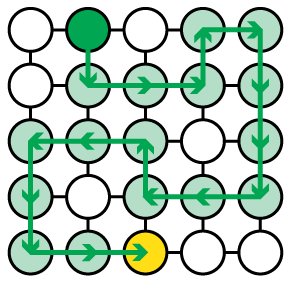
\includegraphics[width=.3\linewidth]{gfx/radius-sat-nav}}

\caption{Affect of wide pheromone trails on node selection}\label{fig:radius-saturation}
\end{figure}

This random behaviour, as far node selection is concerned, has a profound impact on the colony's forage performance, as agents will struggle to find their way to the food sources, and when eventually some of them do, there still a good change that many will not reach the nest back in order to deposit the food they have collected. 

This strongly suggests that ants use more than only local information available at the instant they are making decision where to move to. The other communication methods employed by ants should play a vital role in assisting this decision to be made.

Two new possible experiments to better understand and improve node selection are proposed in section \ref{sec:new-studies}. 

\section{Warning Pheromone Response}
\label{sec:warn-phero-inv}
In this experiment the response of the agents to a warning communication stimulus is tested.

Describe the experiment setup.

Explain that the experiment is done in two phases, the first one the agents react only to amount of warning pheromone and the second one the agents react also to the number of other agents they meet that are traveling in the opposite direction and are not caring food.

Add block diagrams that explain the algorithms the agents use to decide on task selection.

Discuss the results. [experiment not done yet]
Results should vary with the use of different parameters, such as the number of agents traveling in the opposite direction before the agent abort the current task and change to findNestAndHide task.

\chapter{Future Work and Conclusion}
\label{ch:future-work}

\section{Model Improvements}

The model proved to be flexible enough to enable easy implementation of the base classes and the declaration of different agent types and resources. The area that has been least developed is related with simulation. As explained in section \ref{sec:running-sim} there is no formalisation related to simulations. This did not prove to be of any inconvenience during the creation and execution of the simulations for this paper. 

However, for users who are less acquainted with the model and its implementation it could prove to be a challenge to write simulations and collected data from them. More important is the fact that managing all the elements that compose a simulation would be very challenging for the users less experienced to the Java language itself.

\subsection{Simulation handler}

Formalising the simulations and data acquisition by the use of interfaces is necessary. The would remove from the user the responsibility of creation and management of all elements necessary to run simulations. This could be done by the creation of a \emph{simulation handler} that would contain all the necessary data objects, such as the environment (grid of nodes), list of agents, simulation renderers and the necessary methods to schedule data collection, execution of chemical stimulus renderers and so forth.

\subsection{Ant agent navigation improvements}

When it came to implement the different agents from the different casts, the biggest challenge faced was to create an algorithm to take the agents back to their nest. The method implemented in this paper (see sections \ref{sec:ant-memory}, \ref{task:find-home-hide} and \ref{task:find-home-hide}) should be improved in order to be used in more complex and longer simulations. In some cases the simulations would have a high rate of ants not finding their nest at all.

A possible improvement is to bring chemical landmarks to the model. An agent type could be created for this. This type could have properties that would point the ants to the right direction to the nest.

\subsection{Nests As Agents}

As seen in section \ref{sec:ant-nest} nest are represented as agents. On the one hand this facilitates their declaration and use as they enjoy all the infrastructure already in place for agents. On the other hand they are punctual, that is, they are placed in a node as any other agent and the other agents can see their nests only if they reach the same node at which the nest is placed. This is clearly a disadvantage and it does not reflect the reality of natural nests also.

An improvement to the model, that could be used to solve the problem of nests being punctual, could be an new interface to declare \emph{node types}. A node would have a type in the same way agents have. This would open up opportunity to create far more complex environments that it is possible now. For instance, a node could be an  \emph{obstacle} type, agents would not be allowed in there, or even a node could be a chemical landmark. With nodes having types, nests could be modelled as a set of nodes of the \emph{nest type}. This nodes would form a rectangular shape grid, in which if an agent reach any of the nodes they would be able to recognise they have reached their nest.

\section{Implementation Issues}

There is room from improvement on the basic implementation of the model. The comments made in the source files should be consolidated and in some cases improved. However a major possible improvement on the basic implementation is to change the ways the nodes are connected to from the environment grid.  

Currently the nodes are connected in a \emph{four-way} fashion, each node has $4$ neighbours, one in each direction: \emph{north, east, south, west}. This creates a major limitation related to agent navigation. Agents are very unlikely to move in diagonals, as it consists in two movements, first the agent move forward and after it moves sideways. It has been observed that agents hardly would do that because they have very low probability of selecting nodes in a diagonal sequence, e.g. north, east, north, east, north, east. Thus agents generally could not find any food sources in more complex environments where they were not directly aligned to the nest where the ants departed from.

\begin{figure}[H]
\myfloatalign
\subfloat[]
{\label{fig:connection-a}

\includegraphics[width=.2\linewidth]{gfx/connection-4}} \quad
\subfloat[]
{\label{fig:connection-b}
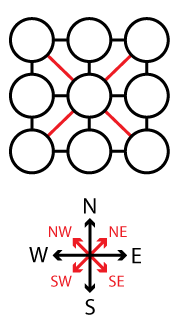
\includegraphics[width=.2\linewidth]{gfx/connection-8}}

\caption{Node connection to its neighbours, four-way connected grid (a) and the eight-way connected grid (b)}
\label{fig:connection}
\end{figure}

An implementation of a grid connected differently would improve the problem considerably. If nodes had $8$ neighbours instead of $4$, agents would be able to navigate directly in the diagonal. Figure \ref{fig:connection} illustrates how the nodes would be connected and all the possible directions the agents could travel towards.

\section{Proposed Studies}
\label{sec:new-studies}

\subsection{Limited Number of Agents Per Node}

This experiment has the potential to explore how the formation and saturation of the pheromone trails would be affected by the limiting the number of agents that can be in a same node at the same time. From the experiment of section \ref{sec:forage-radius-inv} it is clear that in the case of a chemical communication stimulus having radius greater than $0$ agents do not follow a \emph{rational} behaviour towards their goal of foraging. As explained in the experiment discussion the node selection model is responsible for that.

It would be interesting to investigate how the trails would emerge if the nodes had a maximum number of agents allowed in that node at the same time, this would force some agents to move to nodes they would not move to otherwise, it is clear that this is the actual case in nature, as two ants cannot occupy the same physical space. 

\subsection{Improved pheromone sensing capability}

The experiment \emph{Forage Radius Investigation} (Section \ref{sec:forage-radius-inv}) has showed that the agents are too sensitive to the pheromone intensity of the direct neighbours of the node they are currently at. Again, this is due to the node selection model.

This proposed experiment would investigate how the colony forage performance and trail formation would change if agents would take into consideration not only the pheromone intensity of the neighbours of its current node, but also the neighbours of the neighbours. Different 'depths' of sensibility could be experimented. This new feature would reduce the agent's sensibility to direct neighbours of its current node. 

Another possible improvement on the agent's sensing capacity would be the introduction of some sort of memory that would play part of the node selection process.

\section{Conclusion}

The proposed computational model proposed by this paper proved to achieve the two objectives set for this project - flexibility and robustness. The generic model infrastructure provided all the necessary entities to define and implement a wide variety of agents, environments and tasks. More than that, it was possible to demonstrate how simple it is to extend the model, using the case of ant colonies and 2 dimensional environments. Layers of complexity were added as needed, taking advantage of all the previously existing infrastructure with minimal effort.

Also, simulations that were run repeatedly using the same parameters returned, within the expected variations, the same results. The simulations scaled well when the number of agents and the size of the environment varied greatly. Some test experiments used as few as 5 agents in small environments containing a few hundreds of nodes. Some simulations were run for minutes using up to 350 agents in environments containing up to 750,000 nodes with no problems at all.

As far as the implementation of the model is concerned, the model of node selection implemented by this paper was shown to be inappropriate. Further study should be conducted (see section \ref{sec:new-studies} for proposed studies) in order to confirm that. The agents' over-sensitivity to the neighbours of the node it is currently in, is the most problematic effect of the node selection model. The necessity of having to initialise the environment with some pheromone intensity, for the smallest that it might be, is a strong argument against the node selection model implemented by itself. It does not reflect what actually happens in real ant colonies. However this did not affect the two proposed experiments in anyway as their objective was to study how the agents react to the environment changes, starting from a pre-defined setup, whatever it might be.

As for the agent implementation, the problem of taking the agents back to their nest proved to be by far the most challenging task to be implemented. The tasks \emph{FindHomeTask} (section \ref{task:find-home}) and \emph{FindHomeAndHide} (section \ref{task:find-home-hide}) use the agent's limited memory to direct the  agent on its way to the nest, however they proved to be very inefficient and other mechanisms such as chemical landmarks must be considered.

The first experiment demonstrated how agents react to different concentrations of pheromone. The most important outcome of the experiment was the evidence that the trails are a by product of the agents' interactions not only with the environment but also with other agents. They clearly \emph{emerge} from these interactions. This is a case of \emph{strong} emergence. 

Another noteworthy conclusion taken from the first experiment is that the relationship between the quantity of pheromone that each agent deposits in each interaction and the amount of pheromone already present in the environment, regulates the colony's capability to explore the environment around its nest. There is a fine line between having very successful colonies, as far space exploration is concerned, and colonies that could not even reach a source of food. The colony's behaviour switches from one state to another very swiftly depending on this rate.

The second experiment showed that the increase of the communication stimulus' radius did not mean an increase on the forage capacity of the ant colonies, as it was firstly expected. Smaller radiuses give rise to thin, better defined, pheromone trails that allow the agents to move towards the food source direction objectively. Whereas, larger radius 'confuse' the agents within the pheromone trail, seriously undermining the colony's capacity of foraging. The reason for this problem is that communication stimuli with larger radius of reach end up creating clouds of pheromone, and agents have little change to escape this region of high pheromone concentration. This creates a vicious cycle, for the agents in the trail continue to deposit pheromone, over and over again around the same area, saturating the nodes within the trail with pheromone very quickly. Resulting in even smaller probability of 'breaking' from the trail. It is clear that this outcome is also closely related to the agents' over-sensitivity to the pheromone intensity in the neighbour nodes of the current node the agent is in. Once again, this suggests further work to refine the navigational model of node selection would be valuable to improve the model's performance. % Chapter 3
%% Chapter X

\chapter{Chapter Title} % Chapter title

\label{ch:name} % For referencing the chapter elsewhere, use \autoref{ch:name} 

%----------------------------------------------------------------------------------------

\section{Section Title}

Content

%------------------------------------------------

\subsection{Subsection Title}

Content

%------------------------------------------------

\subsection{Subsection Title}

Content

%----------------------------------------------------------------------------------------

\section{Section Title}

Content % Chapter 4 - empty template

%----------------------------------------------------------------------
%	THESIS CONTENT - APPENDICES
%----------------------------------------------------------------------

\appendix

\part{Appendix} % New part of the thesis for the appendix

\chapter{Extra Experimental Results}

I need to select which images to add here. They already have been generated, I just need to choose and crop some of them if necessary.
\chapter{Model and Simulation Source Code}
\label{chapter:model-code}

\section{Ant Model Implementation Details}

The following diagrams show how the ants implementation of the model was extended from the generic part of it. All the ant related entities are coloured in pink.

\begin{figure}[H]
  \centering
  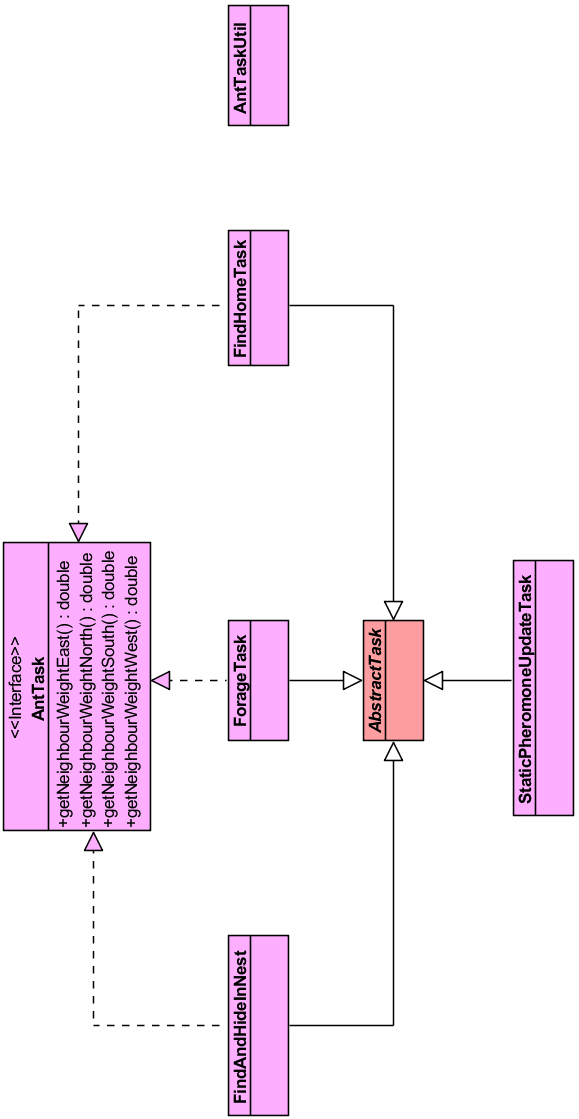
\includegraphics[width=0.55\linewidth]{gfx/ant-task.png}
  \caption{Ant extension of generic task package}
  \label{fig:ant-task}
\end{figure}

\begin{figure}[H]
  \centering
  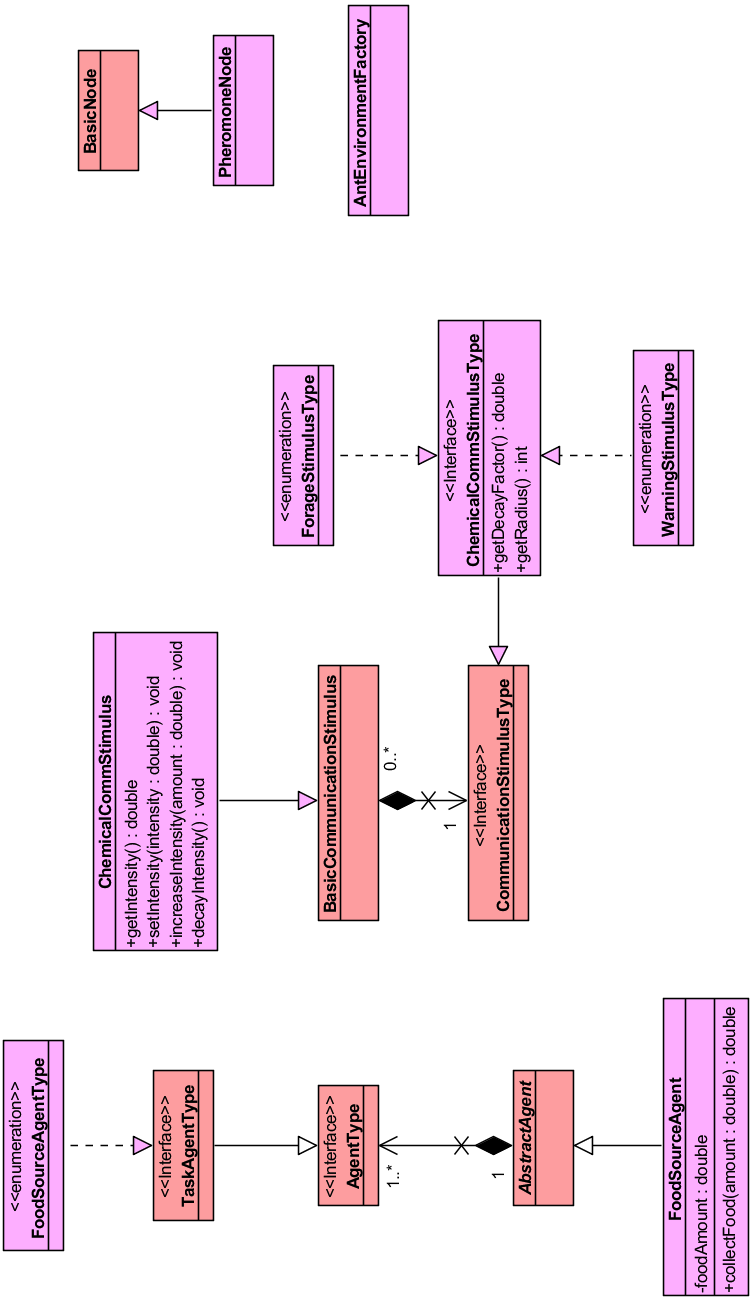
\includegraphics[width=0.8\linewidth]{gfx/ant-env.png}
  \caption{Ant extension of generic environment package}
  \label{fig:ant-env}
\end{figure}

\begin{figure}[H]
  \centering
  \includegraphics[width=0.7\linewidth]{gfx/ant-agent.png}
  \caption{Ant extension of generic agent package}
  \label{fig:ant-agent}
\end{figure}

\section{Source Code}

All the software development was done under a public Git repository available at \url{http://github.com/luizabrahao/msc-project/}. For simplicity, test code has not been included in this section, but it can also be found in the Git repository mentioned, as well as spreadsheets, image source files and other resources used for this project.

\subsection{Environment}
\label{code:env}

\lstinputlisting[label=Node.java,caption=Node.java]{/Users/luiz/Documents/Masters/Project/repository/msc-project/msc-model/src/main/java/com/luizabrahao/msc/model/env/Node.java}

\lstinputlisting[label=BasicNode.java,caption=BasicNode.java]{/Users/luiz/Documents/Masters/Project/repository/msc-project/msc-model/src/main/java/com/luizabrahao/msc/model/env/BasicNode.java}

\lstinputlisting[label=Direction.java,caption=Direction.java]{/Users/luiz/Documents/Masters/Project/repository/msc-project/msc-model/src/main/java/com/luizabrahao/msc/model/env/Direction.java}

\lstinputlisting[label=CommunicationStimulus.java,caption=CommunicationStimulus.java]{/Users/luiz/Documents/Masters/Project/repository/msc-project/msc-model/src/main/java/com/luizabrahao/msc/model/env/CommunicationStimulus.java}

\lstinputlisting[label= CommunicationStimulusType.java,caption= CommunicationStimulusType.java]{/Users/luiz/Documents/Masters/Project/repository/msc-project/msc-model/src/main/java/com/luizabrahao/msc/model/env/CommunicationStimulusType.java}

\lstinputlisting[label= BasicCommunicationStimulus.java,caption= BasicCommunicationStimulus.java]{/Users/luiz/Documents/Masters/Project/repository/msc-project/msc-model/src/main/java/com/luizabrahao/msc/model/env/BasicCommunicationStimulus.java}

\lstinputlisting[label= FoodSourceAgentType.java,caption= FoodSourceAgentType.java]{/Users/luiz/Documents/Masters/Project/repository/msc-project/msc-model/src/main/java/com/luizabrahao/msc/ants/env/FoodSourceAgentType.java}

\lstinputlisting[label= FoodSourceAgent.java,caption= FoodSourceAgent.java]{/Users/luiz/Documents/Masters/Project/repository/msc-project/msc-model/src/main/java/com/luizabrahao/msc/ants/env/FoodSourceAgent.java}

\lstinputlisting[label= PheromoneNode.java,caption= PheromoneNode.java]{/Users/luiz/Documents/Masters/Project/repository/msc-project/msc-model/src/main/java/com/luizabrahao/msc/ants/env/PheromoneNode.java}

\lstinputlisting[label= ForageStimulusType.java,caption= ForageStimulusType.java]{/Users/luiz/Documents/Masters/Project/repository/msc-project/msc-model/src/main/java/com/luizabrahao/msc/ants/env/ForageStimulusType.java}

\lstinputlisting[label= WarningStimulusType.java,caption= WarningStimulusType.java]{/Users/luiz/Documents/Masters/Project/repository/msc-project/msc-model/src/main/java/com/luizabrahao/msc/ants/env/WarningStimulusType.java}

\subsection{Agent}
\label{code:agent}

\lstinputlisting[label= Agent.java,caption= Agent.java]{/Users/luiz/Documents/Masters/Project/repository/msc-project/msc-model/src/main/java/com/luizabrahao/msc/model/agent/Agent.java}

\lstinputlisting[label= AbstractAgent.java,caption= AbstractAgent.java]{/Users/luiz/Documents/Masters/Project/repository/msc-project/msc-model/src/main/java/com/luizabrahao/msc/model/agent/AbstractAgent.java}

\lstinputlisting[label= TaskAgent.java,caption= TaskAgent.java]{/Users/luiz/Documents/Masters/Project/repository/msc-project/msc-model/src/main/java/com/luizabrahao/msc/model/agent/TaskAgent.java}

\lstinputlisting[label= AgentType.java,caption= AgentType.java]{/Users/luiz/Documents/Masters/Project/repository/msc-project/msc-model/src/main/java/com/luizabrahao/msc/model/agent/AgentType.java}

\lstinputlisting[label= TaskAgentType.java,caption= TaskAgentType.java]{/Users/luiz/Documents/Masters/Project/repository/msc-project/msc-model/src/main/java/com/luizabrahao/msc/model/agent/TaskAgentType.java}

\lstinputlisting[label= BasicTaskAgentType.java,caption= BasicTaskAgentType.java]{/Users/luiz/Documents/Masters/Project/repository/msc-project/msc-model/src/main/java/com/luizabrahao/msc/model/agent/BasicTaskAgentType.java}

\lstinputlisting[label= Ant.java,caption= Ant.java]{/Users/luiz/Documents/Masters/Project/repository/msc-project/msc-model/src/main/java/com/luizabrahao/msc/ants/agent/Ant.java}

\lstinputlisting[label= AntAgent.java,caption= AntAgent.java]{/Users/luiz/Documents/Masters/Project/repository/msc-project/msc-model/src/main/java/com/luizabrahao/msc/ants/agent/AntAgent.java}

\lstinputlisting[label= AntType.java,caption= AntType.java]{/Users/luiz/Documents/Masters/Project/repository/msc-project/msc-model/src/main/java/com/luizabrahao/msc/ants/agent/AntType.java}

\lstinputlisting[label= WorkerAntType.java,caption= WorkerAntType.java]{/Users/luiz/Documents/Masters/Project/repository/msc-project/msc-model/src/main/java/com/luizabrahao/msc/ants/agent/WorkerAntType.java}

\lstinputlisting[label= AntNestType.java,caption= AntNestType.java]{/Users/luiz/Documents/Masters/Project/repository/msc-project/msc-model/src/main/java/com/luizabrahao/msc/ants/agent/AntNestType.java}

\lstinputlisting[label= AntNestAgent.java,caption= AntNestAgent.java]{/Users/luiz/Documents/Masters/Project/repository/msc-project/msc-model/src/main/java/com/luizabrahao/msc/ants/agent/AntNestAgent.java}

\lstinputlisting[label= StaticPheromoneUpdaterAgentType.java,caption= StaticPheromoneUpdaterAgentType.java]{/Users/luiz/Documents/Masters/Project/repository/msc-project/msc-model/src/main/java/com/luizabrahao/msc/ants/agent/StaticPheromoneUpdaterAgentType.java}

\lstinputlisting[label= StaticPheromoneUpdaterAgent.java,caption= StaticPheromoneUpdaterAgent.java]{/Users/luiz/Documents/Masters/Project/repository/msc-project/msc-model/src/main/java/com/luizabrahao/msc/ants/agent/StaticPheromoneUpdaterAgent.java}

\subsection{Task}
\label{code:task}

\lstinputlisting[label= Task.java,caption= Task.java]{/Users/luiz/Documents/Masters/Project/repository/msc-project/msc-model/src/main/java/com/luizabrahao/msc/model/task/Task.java}

\lstinputlisting[label= AbstractTask.java,caption= AbstractJava.java]{/Users/luiz/Documents/Masters/Project/repository/msc-project/msc-model/src/main/java/com/luizabrahao/msc/model/task/AbstractTask.java}

\lstinputlisting[label= WandererTask.java,caption= WandererTask.java]{/Users/luiz/Documents/Masters/Project/repository/msc-project/msc-model/src/main/java/com/luizabrahao/msc/model/task/WandererTask.java}


\lstinputlisting[label= AntTask.java,caption= AntTask.java]{/Users/luiz/Documents/Masters/Project/repository/msc-project/msc-model/src/main/java/com/luizabrahao/msc/ants/task/AntTask.java}

\lstinputlisting[label= ForageTask.java,caption= ForageTask.java]{/Users/luiz/Documents/Masters/Project/repository/msc-project/msc-model/src/main/java/com/luizabrahao/msc/ants/task/ForageTask.java}

\lstinputlisting[label= FindHomeTask.java,caption= FindHomeTask.java]{/Users/luiz/Documents/Masters/Project/repository/msc-project/msc-model/src/main/java/com/luizabrahao/msc/ants/task/FindHomeTask.java}

\lstinputlisting[label= FindHomeHideInNest.java,caption= FinAndHideInNest.java]{/Users/luiz/Documents/Masters/Project/repository/msc-project/msc-model/src/main/java/com/luizabrahao/msc/ants/task/FindAndHideInNest.java}

\lstinputlisting[label= AntTaskUtil.java,caption= AntTaskUtil.java]{/Users/luiz/Documents/Masters/Project/repository/msc-project/msc-model/src/main/java/com/luizabrahao/msc/ants/task/AntTaskUtil.java}

\lstinputlisting[label= StaticPheromoneUpdateTask.java,caption= StaticPheromoneUpdateTask.java]{/Users/luiz/Documents/Masters/Project/repository/msc-project/msc-model/src/main/java/com/luizabrahao/msc/ants/task/StaticPheromoneUpdateTask.java}

\subsection{Annotations}
\label{code:annotations}

\lstinputlisting[label= FrameworkExclusive.java,caption= FrameworkExclusive.java]{/Users/luiz/Documents/Masters/Project/repository/msc-project/msc-model/src/main/java/com/luizabrahao/msc/model/annotation/FrameworkExclusive.java}

\lstinputlisting[label= PseudoThreadSafe.java,caption= PseudoThreadSafe.java]{/Users/luiz/Documents/Masters/Project/repository/msc-project/msc-model/src/main/java/com/luizabrahao/msc/model/annotation/PseudoThreadSafe.java}

\lstinputlisting[label= ThreadSafetyBreaker.java,caption= ThreadSafetyBreaker.java]{/Users/luiz/Documents/Masters/Project/repository/msc-project/msc-model/src/main/java/com/luizabrahao/msc/model/annotation/ThreadSafetyBreaker.java}

\subsection{Utility}

\lstinputlisting[label=EnvironmentFactory,caption=EnvironmentFactory.java]{/Users/luiz/Documents/Masters/Project/repository/msc-project/msc-model/src/main/java/com/luizabrahao/msc/model/env/EnvironmentFactory.java}

\lstinputlisting[label= AntEnvironmentFactory.java,caption= AntEnvironmentFactory.java]{/Users/luiz/Documents/Masters/Project/repository/msc-project/msc-model/src/main/java/com/luizabrahao/msc/ants/env/AntEnvironmentFactory.java}

\lstinputlisting[label= AntAgentFactory.java,caption= AntAgentFactory.java]{/Users/luiz/Documents/Masters/Project/repository/msc-project/msc-model/src/main/java/com/luizabrahao/msc/ants/agent/AntAgentFactory.java}

\subsection{Simulation Renderers}

\lstinputlisting[label= ExploredSpaceRenderer.java,caption= ExploredSpaceRenderer.java]{/Users/luiz/Documents/Masters/Project/repository/msc-project/msc-model/src/main/java/com/luizabrahao/msc/ants/render/ExploredSpaceRenderer.java}

\lstinputlisting[label= NodeHistoryRenderer.java,caption= ExploredSpaceRenderer.java]{/Users/luiz/Documents/Masters/Project/repository/msc-project/msc-model/src/main/java/com/luizabrahao/msc/ants/render/NodeHistoryRenderer.java}

\lstinputlisting[label= PheromoneRenderer.java,caption= PheromoneRenderer.java]{/Users/luiz/Documents/Masters/Project/repository/msc-project/msc-model/src/main/java/com/luizabrahao/msc/ants/render/PheromoneRenderer.java}

\lstinputlisting[label= PopulationRenderer.java,caption= PopulationRenderer.java]{/Users/luiz/Documents/Masters/Project/repository/msc-project/msc-model/src/main/java/com/luizabrahao/msc/ants/render/PopulationRenderer.java}

\subsection{Simlations}

\lstinputlisting[label= PathSimulation.java,caption= PathSimulation.java]{/Users/luiz/Documents/Masters/Project/repository/msc-project/msc-model/src/test/java/com/luizabrahao/msc/simulations/PathSimulation.java}

\lstinputlisting[label= StudyOnRadius.java,caption= StudyOnRadius.java]{/Users/luiz/Documents/Masters/Project/repository/msc-project/msc-model/src/test/java/com/luizabrahao/msc/simulations/StudyOnRadius.java}



%----------------------------------------------------------------------
%	POST-CONTENT THESIS PAGES
%----------------------------------------------------------------------

\cleardoublepage% Bibliography

\label{app:bibliography} % Reference the bibliography elsewhere with \autoref{app:bibliography}

\manualmark
\markboth{\spacedlowsmallcaps{\bibname}}{\spacedlowsmallcaps{\bibname}} 
\refstepcounter{dummy}

\addtocontents{toc}{\protect\vspace{\beforebibskip}} % Place the bibliography slightly below the rest of the document content in the table of contents
\addcontentsline{toc}{chapter}{\tocEntry{\bibname}}

\bibliographystyle{plainnat}

\bibliography{Bibliography} % Bibliography

%----------------------------------------------------------------------
\end{addmargin}
\end{document}
